% IEEE Access submission version of the manuscript.
% Uses IEEEtran (journal mode) as a stand-in for ieeeaccess.cls;
% the official Access template is a thin wrapper around IEEEtran.
% IEEEtran.cls and IEEEtran.bst are checked in to this directory so
% the file compiles without modifying the system TeX installation.
\documentclass[journal]{IEEEtran}

\usepackage[T1]{fontenc}
\usepackage[utf8]{inputenc}
\usepackage{microtype}
\usepackage{graphicx}
\usepackage{booktabs}
\usepackage{amsmath}
\usepackage{amssymb}
\usepackage{multirow}
\usepackage{subcaption}
\usepackage{cite}
\usepackage[numbers,sort&compress]{natbib}
\usepackage{hyperref}
\usepackage{url}
% Defensive stubs: if Overleaf's TeX Live has lineno hooks left over from a
% prior compile of the ACL version (main.tex uses acl.sty which loads lineno),
% \@LN@col can appear in the aux file and break a fresh main_ieee compile.
% These no-op definitions absorb the call without affecting layout.
\makeatletter
\providecommand{\@LN@col}[1]{}
\providecommand{\linenumbers}{}
\providecommand{\nolinenumbers}{}
\makeatother
\newcommand{\far}{\mathrm{FAR}}
\newcommand{\tar}{\mathrm{TAR}}

\title{When the Interface Changes the Verdict:\\Measurement Brittleness in LLM Critique}

\author{
  First~Author,~\IEEEmembership{Member,~IEEE,}
  and~Second~Author,~\IEEEmembership{Member,~IEEE}%
  \thanks{The authors are with the Affiliation.
          E-mail: email@domain.}
}

\markboth{IEEE Access, Vol.~XX, No.~Y, Month~2026}%
{Author \MakeLowercase{\textit{et al.}}: Measurement Brittleness in LLM Critique}

\begin{document}
\maketitle

\begin{abstract}
Large language models (LLMs) are increasingly used as judges for benchmark construction, model selection, and critique-repair pipelines. These evaluations usually specify the judge model, but they often leave the judge-side output interface under-specified. This paper studies whether benign interface choices, such as rubric structure, score-versus-verdict order, schema field order, and repair coupling, can act as a measurement confound. Holding judged content fixed and using constrained decoding, we compare multiple judge models across reasoning datasets under several common output interfaces. We find that interface choices do more than shift absolute accuracy: they can change pairwise judge gaps, alter adjacent model orderings, and mask task-specific reversals when results are pooled. The effect is not uniform across models or datasets, which is precisely the methodological risk for LLM-as-judge comparisons. We also observe that verdict changes occur at the item level, especially on wrong candidate solutions, rather than only as aggregate noise. A secondary ablation suggests that adding an explicit deliberation field to the output contract can reduce interface sensitivity in the tested setting, but this should be understood as another interface design choice rather than a general solution. Together, these results characterize a form of interface-dependent measurement variation in LLM-as-judge evaluation. They suggest that some reported judge differences may partly reflect the output contract used to elicit the verdict, motivating analyses that report the judge interface and check whether model comparisons are stable under reasonable interface variants.
\end{abstract}

\begin{IEEEkeywords}
LLM-as-a-judge, model evaluation, prompt sensitivity, structured output, critique systems, measurement validity.
\end{IEEEkeywords}

\section{Introduction}
\label{sec:intro}

Large language models are now routinely used to evaluate other model outputs. They grade benchmark answers, select among system variants, provide feedback for refinement pipelines, and stand in for human preference annotators when human evaluation is too slow or expensive \citep{liu2023geval, zheng2024judging, kim2024prometheus, lambert2024rewardbench}. In these settings, the judge model is usually named and compared, while the judge-side interface is treated as a prompt-engineering detail. A leaderboard may report that judge model A is more reliable than judge model B under one rubric, output schema, or scoring protocol, and leave open whether the same conclusion would hold under another benign interface.

This paper studies that gap. We define a judge-side output interface as the response contract imposed on the judge: whether it emits a free verdict or rubric checklist, whether it gives a score before or after a binary verdict, whether the schema contains a correction field, and whether a requested correction is produced before or after the verdict. These choices are benign in the sense that they do not adversarially perturb the candidate answer being judged. They are also common: production evaluation code often asks judges for JSON, confidence scores, explanations, rubrics, or repairs in a single call.

The claim is not simply that LLMs are prompt-sensitive. General prompt-format sensitivity is already well established \citep{sclar2024spurious, mizrahi2024multiprompt}, and LLM-as-judge work has documented position, length, provenance, safety-prompt, and protocol effects \citep{zheng2024judging, dubois2024length, eiras2025know, zhang2026judgeconfig, tripathi2025pairwise}. We treat these results as the starting point, not the novelty claim. The narrower question here is whether benign judge-side output interfaces preserve the comparison between judge models when the judged content is fixed. If each judge model responded to interface changes in the same way, model comparisons might shift in absolute level while preserving conclusions. The methodological risk arises when interface sensitivity differs by judge model: the estimated gap between judges, the statistical significance of that gap, or even the ranking of adjacent judges can change under fixed judged content.

We therefore hold the judged content fixed. Each judge sees the same problem, the same candidate solution, and the same ground-truth-checkable task instance; only the judge-side interface changes. We use constrained decoding for the final verdict object so that literal JSON parse failures do not drive the main comparison. Parser-aware replay remains part of the methodology, but as an audit: it distinguishes behavioral interface effects from measurement artifacts when structured outputs fail. The primary estimand is the judge-model by interface interaction, measured through false-accept rate, false-reject rate, balanced accuracy, pairwise judge gaps, and interface-specific rankings.

Repair coupling is the most distinctive interface axis in this study. Self-refinement and critique-repair systems ask whether feedback and revision improve a generated answer \citep{madaan2023selfrefine, gou2024critic, lin2024criticbench}. We ask a different question: whether asking the judge to repair a candidate solution changes the verdict used to decide whether repair is needed in the first place. A verdict-first interface, a repair-coupled interface, and a repair-then-verdict interface are not merely cosmetic variants if they induce different judge policies.

As a preliminary motivation for the final experiments, an AIME pilot with three local judge configurations found that a repair-then-verdict interface can change the top adjacent comparison under balanced accuracy, while other interfaces preserve the opposite ordering. The finalized Results section will report the full multi-dataset analysis after all runs are frozen; the point here is the design principle. A single judge interface is not a neutral lens on judge ability unless this invariance is tested.

The article makes four contributions. First, it isolates benign judge-side output-interface choices under fixed judged content and constrained decoding, separating this question from general prompt sensitivity, response-side perturbation, and single-judge stability work. Second, it tests judge-model by interface interactions directly, using model-comparison stability rather than only absolute judge accuracy as the target. Third, it studies repair coupling and repair/verdict order as evaluation-interface variables, a setting not addressed by standard self-refinement studies that focus on whether the final solution improves. Fourth, it treats parser-aware replay and non-verdict accounting as methodological safeguards rather than headline effects, clarifying when structured-output artifacts do or do not explain observed interface sensitivity.

\section{Background and Related Work}
\label{sec:related}

\subsection{LLM-as-Judge Evaluation and Protocol Confounds}
\label{sec:rw-judge}

LLM-as-judge systems use language models to evaluate candidate outputs, often replacing or augmenting human evaluation. G-Eval used chain-of-thought and form-filling to align GPT-4-based evaluation with human judgments on generation tasks \citep{liu2023geval}. MT-Bench and Chatbot Arena popularized model-based judging for open-ended chat evaluation and documented important judge biases, including position and verbosity effects \citep{zheng2024judging}. AlpacaEval made similar automatic evaluation practical at scale, and Length-Controlled AlpacaEval showed that even a single response-side confound, output length, can substantially distort automatic win rates unless explicitly controlled \citep{dubois2024length}. Prometheus and RewardBench further illustrate how evaluator models, rubrics, and reward-model benchmarks have become part of the infrastructure for comparing systems \citep{kim2024prometheus, lambert2024rewardbench}. Safety-judge robustness work similarly shows that judge decisions can be sensitive to style and adversarial perturbations in the judged output \citep{eiras2025know}.

These studies establish that LLM-as-judge evaluation is not a simple readout of latent response quality. They do not, however, isolate the judge-side output interface while holding judged content fixed. Our focus is not whether a candidate answer is longer, more adversarially phrased, or attributed to a different source. It is whether the response contract imposed on the judge changes the measurement of judge reliability and changes comparisons among judge models.

Recent meta-evaluation work studies related but distinct protocol sensitivities. JudgeSense measures per-judge sensitivity to semantically equivalent prompt paraphrases, providing a single-judge stability benchmark rather than testing whether the same interface perturbation changes cross-judge model comparisons \citep{bellibatlu2026judgesense}. Zhang studies safety benchmark sensitivity to judge prompt wording, finding harmful-rate shifts up to 24.2 percentage points and moderately stable safety rankings under one main safety-classification setting \citep{zhang2026judgeconfig}. Tripathi et al.\ compare pairwise and pointwise feedback protocols and show that protocol choice affects bias and preference stability, with pairwise preferences flipping much more often than pointwise judgments under their perturbations \citep{tripathi2025pairwise}. These papers make prompt and protocol sensitivity unsurprising. Our experiment targets a different object: benign judge-side output-interface choices under fixed judged content, constrained decoding, and objective ground truth, with the judge-model by interface interaction as the primary estimand.

\subsection{Prompt Sensitivity Versus Interface Interaction}
\label{sec:rw-prompt-format}

General LLM prompt sensitivity is well known. Sclar et al.\ show that seemingly spurious formatting choices can strongly affect model performance and do not transfer uniformly across models \citep{sclar2024spurious}. Mizrahi et al.\ argue that single-prompt evaluation is brittle and call for multi-prompt evaluation across models and tasks \citep{mizrahi2024multiprompt}. These results motivate caution, but they are broader than our claim. A model can be prompt-sensitive without invalidating a model comparison if all compared models shift similarly. Conversely, even moderate absolute shifts can become consequential when they differ by judge and change adjacent pairwise comparisons.

The present study targets the interaction. We ask whether judge models respond differently to benign output-interface choices, so that the estimated gap between judges changes with the interface. The relevant object is therefore not only the variance of a single model across prompts, but the judge-model by interface term: schema shape, field order, score/verdict order, rubric structure, and repair coupling may induce different policies in different judges. This interaction is what makes an unreported judge interface a leaderboard confound.

\subsection{Structured Outputs and Reasoning Under Constraints}
\label{sec:rw-structured}

Structured generation is widely used because evaluation pipelines need parseable fields. G-Eval's form-filling paradigm and Prometheus's rubric-conditioned evaluator are early examples of evaluation designs in which the response contract is part of the judge protocol \citep{liu2023geval, kim2024prometheus}. Tam et al.\ show that format restrictions such as JSON or XML can reduce LLM performance on reasoning and knowledge tasks, with stricter constraints often degrading performance more \citep{tam2024speak}. This is directly relevant because LLM-as-judge systems often require structured verdicts, scores, rationales, and corrections.

Our design differs in two ways. First, we use constrained decoding to prevent literal JSON failures from dominating the main estimates. Second, we compare multiple structured interfaces under the same judged content. The question is not only whether structure hurts a single model, but whether alternative structured interfaces change the relative measured reliability of different judge models.

\subsection{Calibration and Confidence Reporting}
\label{sec:rw-calibration}

Many LLM judges report confidence or scalar scores, and prior work has shown that elicited confidence can be poorly calibrated even when models are explicitly asked for calibrated probabilities \citep{tian2023justask}. We do not claim that LLM overconfidence is new. In this paper, confidence is a secondary measurement channel used to ask whether the output interface changes calibration behavior alongside verdict behavior. This makes calibration evidence supportive of the interface-interaction analysis, rather than a standalone contribution.

\subsection{Source Bias, Self-Preference, and Judged-Content Perturbations}
\label{sec:rw-source}

Another line of work studies how the judged content or its attribution affects evaluation. LLM judges can show self-preference or source-framing effects, favoring outputs generated by themselves, familiar model families, or particular stated sources \citep{panickssery2024selfpreference, wataoka2024selfpreference, germani2025sourceframing}. These effects matter for benchmark design, but they manipulate the candidate answer, its provenance, or the metadata attached to it.

We treat this literature as a contrast case. The present experiments keep the judged content anonymous and fixed. The candidate solution does not change, the solver identity is hidden, and the ground-truth label is fixed before judging. This lets us isolate the judge-side interface rather than a source label or response-side feature.

\subsection{Critique-Repair Pipelines}
\label{sec:rw-pipelines}

Self-correction and critique-repair methods ask whether feedback improves the final answer. Self-Refine uses iterative self-feedback and revision \citep{madaan2023selfrefine}; CRITIC adds tool-interactive feedback to support self-correction \citep{gou2024critic}; CriticBench evaluates critique-correct reasoning abilities across tasks and models \citep{lin2024criticbench}. These studies focus on the quality of the revised solution or the ability to generate useful feedback.

Our repair-coupling axis asks a different measurement question. In judge pipelines, the verdict often gates whether repair should happen at all. If a prompt asks the judge to both decide correctness and produce a corrected answer, the repair task may change the verdict itself. A repair-then-verdict interface is therefore not just a different repair strategy; it is a different judge measurement protocol. This distinction is especially important for leaderboards that compare judge models by verdict accuracy but do not standardize the repair or output contract.

\subsection{Reasoning and Deliberation in Judge Interfaces}
\label{sec:rw-deliberation}

Reasoning traces and chain-of-thought prompting can improve some reasoning tasks \citep{wei2022cot}, but structured-output constraints can suppress or reshape how models externalize reasoning. The present study therefore treats reasoning as an interface variable rather than as an unobserved native capability. In the deliberation-in-schema robustness ablation, the judge is given an explicit reasoning field before the verdict inside the same constrained output object. This tests whether adding a controlled deliberation slot stabilizes judge comparisons across interfaces. It is not interpreted as a claim about private native chain-of-thought.

\section{Methods}
\label{sec:methods}

\subsection{Task Setting}
\label{sec:task-setting}

Each experimental unit consists of a problem, a fixed candidate solution, a ground-truth answer, a judge model, and a judge-side output interface. The candidate solution includes the solver's reasoning trace and final answer. The judge receives the same problem and candidate solution in every interface arm and returns a constrained structured verdict. The primary verdict outcome is whether the judge marks the solution as correct. For actually wrong candidate solutions, marking the solution as correct is a false accept. For actually correct candidate solutions, marking it as wrong is a false reject.

The distinction between wrong and correct candidate solutions is determined before judging using dataset-specific answer checking. This fixed-content design isolates the judge-model by interface interaction: only the judge output contract changes, while the judged content, ground truth, source attribution, and candidate correctness label remain fixed. All main interface-confound runs use anonymous source attribution.

\subsection{Datasets}
\label{sec:datasets}

Experiments use four reasoning datasets that differ in domain and answer format. AIME contains competition mathematics problems with short numeric answers. GPQA contains graduate-level scientific multiple-choice questions designed to require expert knowledge \citep{rein2023gpqa}. MMLU-Pro is used as a broad multiple-choice reasoning benchmark with a more challenging and prompt-robust design than the original MMLU \citep{wang2024mmlupro}. Olympiad contains challenging mathematical problems drawn from OlympiadBench \citep{he2024olympiadbench}. This objective-answer setting follows the same motivation as benchmarks such as LiveBench, which avoid subjective LLM judging when automatic ground-truth scoring is available \citep{white2024livebench}.

For each dataset, we sample 75 cached candidate solutions using seed 42: 50 actually wrong candidates and 25 actually correct candidates. Candidate identifiers are shuffled once before selection. The same 75 candidates are evaluated by every judge-interface cell. Before judging, candidate solutions that alone exceed the shared 32k context window are removed as uniform content-driven exclusions. The exclusions are identical across all judge and interface cells within a dataset: 9 AIME problem identifiers, 4 GPQA identifiers, 3 MMLU-Pro identifiers, and 10 Olympiad identifiers. The resulting analyzable pools contain 66, 71, 72, and 65 candidates, respectively, before any judge-specific non-verdicts.

\subsection{Solver and Critic Models}
\label{sec:models}

The no-deliberation matrix uses three local judge configurations: Gemma-4-no-think, gpt-oss-no-think, and qwen3-no-think. Each judge evaluates every dataset under every output interface, yielding 4500 attempted judgments before uniform context exclusions and transient non-verdicts: three judges, four datasets, five interfaces, and 75 candidate solutions per dataset.

All judges are served through the repository's local model presets. qwen3-no-think uses Qwen/Qwen3-32B with enable\_thinking=False; gpt-oss-no-think uses openai/gpt-oss-20b with reasoning\_effort=low; Gemma-4-no-think uses the Gemma-4 local serving configuration. The interface-confound runs use constrained JSON decoding through response\_format=json\_schema with strict schemas and a judge completion budget of max\_tokens=16000. The default endpoint is http://localhost:8000/v1.

The secondary deliberation-in-schema run uses the same three judge families on AIME and GPQA. It does not rely on native private chain-of-thought modes. Instead, the constrained schema adds a required leading free-text reasoning field before the verdict fields, paired with an instruction to think step by step before emitting the verdict. This makes deliberation an explicit output-interface intervention.

\subsection{Prompt-Interface Variants}
\label{sec:prompt-variants}

The no-deliberation matrix uses five benign output interfaces. \textsc{Verdict-Only} asks for a binary correctness verdict and confidence. \textsc{Rubric-Verdict} asks the judge to evaluate a short rubric before returning the verdict. \textsc{Score-Then-Verdict} asks for a score before the binary verdict. \textsc{Verdict+Repair} asks for the verdict before a corrected answer field. \textsc{Repair-Then-Verdict} asks for the corrected answer field before the verdict. These variants change the judge-side response contract, not the judged content.

\subsection{Logging Schema and Answer Checking}
\label{sec:logging}

Each judgment record stores the dataset, problem identifier, candidate identifier, judge model, output interface, parsed verdict, confidence when present, corrected answer when requested, raw response, token counts, non-verdict status, and the precomputed correctness of the candidate solution. Ground-truth checking uses dataset-specific answer normalization. For short-answer mathematics datasets, the final answer is normalized before exact or symbolic comparison. For multiple-choice datasets, the selected option is compared against the answer key. The main interface-confound analysis uses the verdict only; corrected answers are logged for secondary repair analyses.

\subsection{Coverage and Non-Verdict Handling}
\label{sec:parse-handling}

Constrained decoding removes the literal malformed-JSON artifact from the main experiment, but a judge call can still fail to yield an analyzable verdict because the candidate solution exceeds the context window, the completion is truncated, or the serving request errors. We log these cases separately as ctx\_overflow, length\_trunc, error, or other. Context-overflow exclusions are determined before judging and are uniform across all judge-interface cells within a dataset. Verdict metrics are computed on valid verdicts after these exclusions. We report valid-verdict coverage on the analyzable pool so that interface effects can be separated from coverage effects.

\subsection{Metrics}
\label{sec:metrics}

The primary metrics are false-accept rate (FAR), false-reject rate (FRR), and balanced accuracy. FAR is the fraction of actually wrong candidate solutions judged correct. FRR is the fraction of actually correct candidate solutions judged wrong. Balanced accuracy is the average of wrong-item rejection rate and correct-item acceptance rate:
\begin{equation}
\mathrm{BAcc} = \frac{1}{2}\left[(1-\far) + (1-\mathrm{FRR})\right].
\end{equation}
Model comparisons use balanced accuracy because the candidate pool is intentionally enriched for wrong solutions.

For leaderboard stability, we compute judge rankings within each dataset-interface cell, pairwise balanced-accuracy gaps between judges, and Kendall rank correlations between interface-specific judge rankings. For item-level instability, we compute the fraction of fixed candidates whose verdict changes across interfaces under the same judge.

\subsection{Statistical Analysis}
\label{sec:stats}

All pairwise judge comparisons are item-paired within an interface and dataset. We report absolute balanced-accuracy gaps in percentage points with cluster-bootstrap 95\% confidence intervals \citep{efron1993bootstrap}, resampling problem identifiers and retaining all candidate rows associated with a resampled problem. This clustering handles the small number of cases where the same problem appears with both a wrong and a correct candidate solution.

For model-based inference, we fit generalized estimating equation (GEE) binomial logistic regressions for verdict correctness \citep{liang1986longitudinal}. The per-dataset models include judge, interface, and judge-by-interface terms and cluster by problem identifier. We also fit a pooled two-way model with dataset fixed effects and judge-by-interface terms. Finally, to test whether the judge-by-interface interaction changes across task families, we fit a pooled three-way model with judge, interface, dataset, and judge-by-interface-by-dataset terms, clustering by dataset-specific problem identifier. The joint robust Wald test on the 24 three-way interaction terms is the pre-specified test for task-dependent interface confounding. The frozen GEE summary is stored in the paper's tables directory, and the analysis is generated by the interface-confound, item-disagreement, and think-versus-no-think scripts.



\section{Results}
\label{sec:results}

\subsection{Interface Choices Change Judge Comparisons Within Task Families}
\label{sec:results-within-task}

The fixed-content interface matrix shows the target interaction directly. The same candidate solutions produce different judge rankings when only the judge-side output contract changes. This is not a single-dataset anomaly. In per-dataset GEE models of verdict correctness, the judge-by-interface block contains significant interaction terms in all four task families: 6 on AIME, 3 on GPQA, 2 on Olympiad, and 1 on MMLU-Pro. These counts are frozen in paper/tables/ifc\_gee\_summary.csv. Figure~\ref{fig:ifc-heatmap} visualizes the per-dataset judge-interface matrix, and Table~\ref{tab:ifc-dataset-summary} summarizes the ranking instability seen in the frozen per-dataset artifacts.

\begin{figure*}[t]
\centering
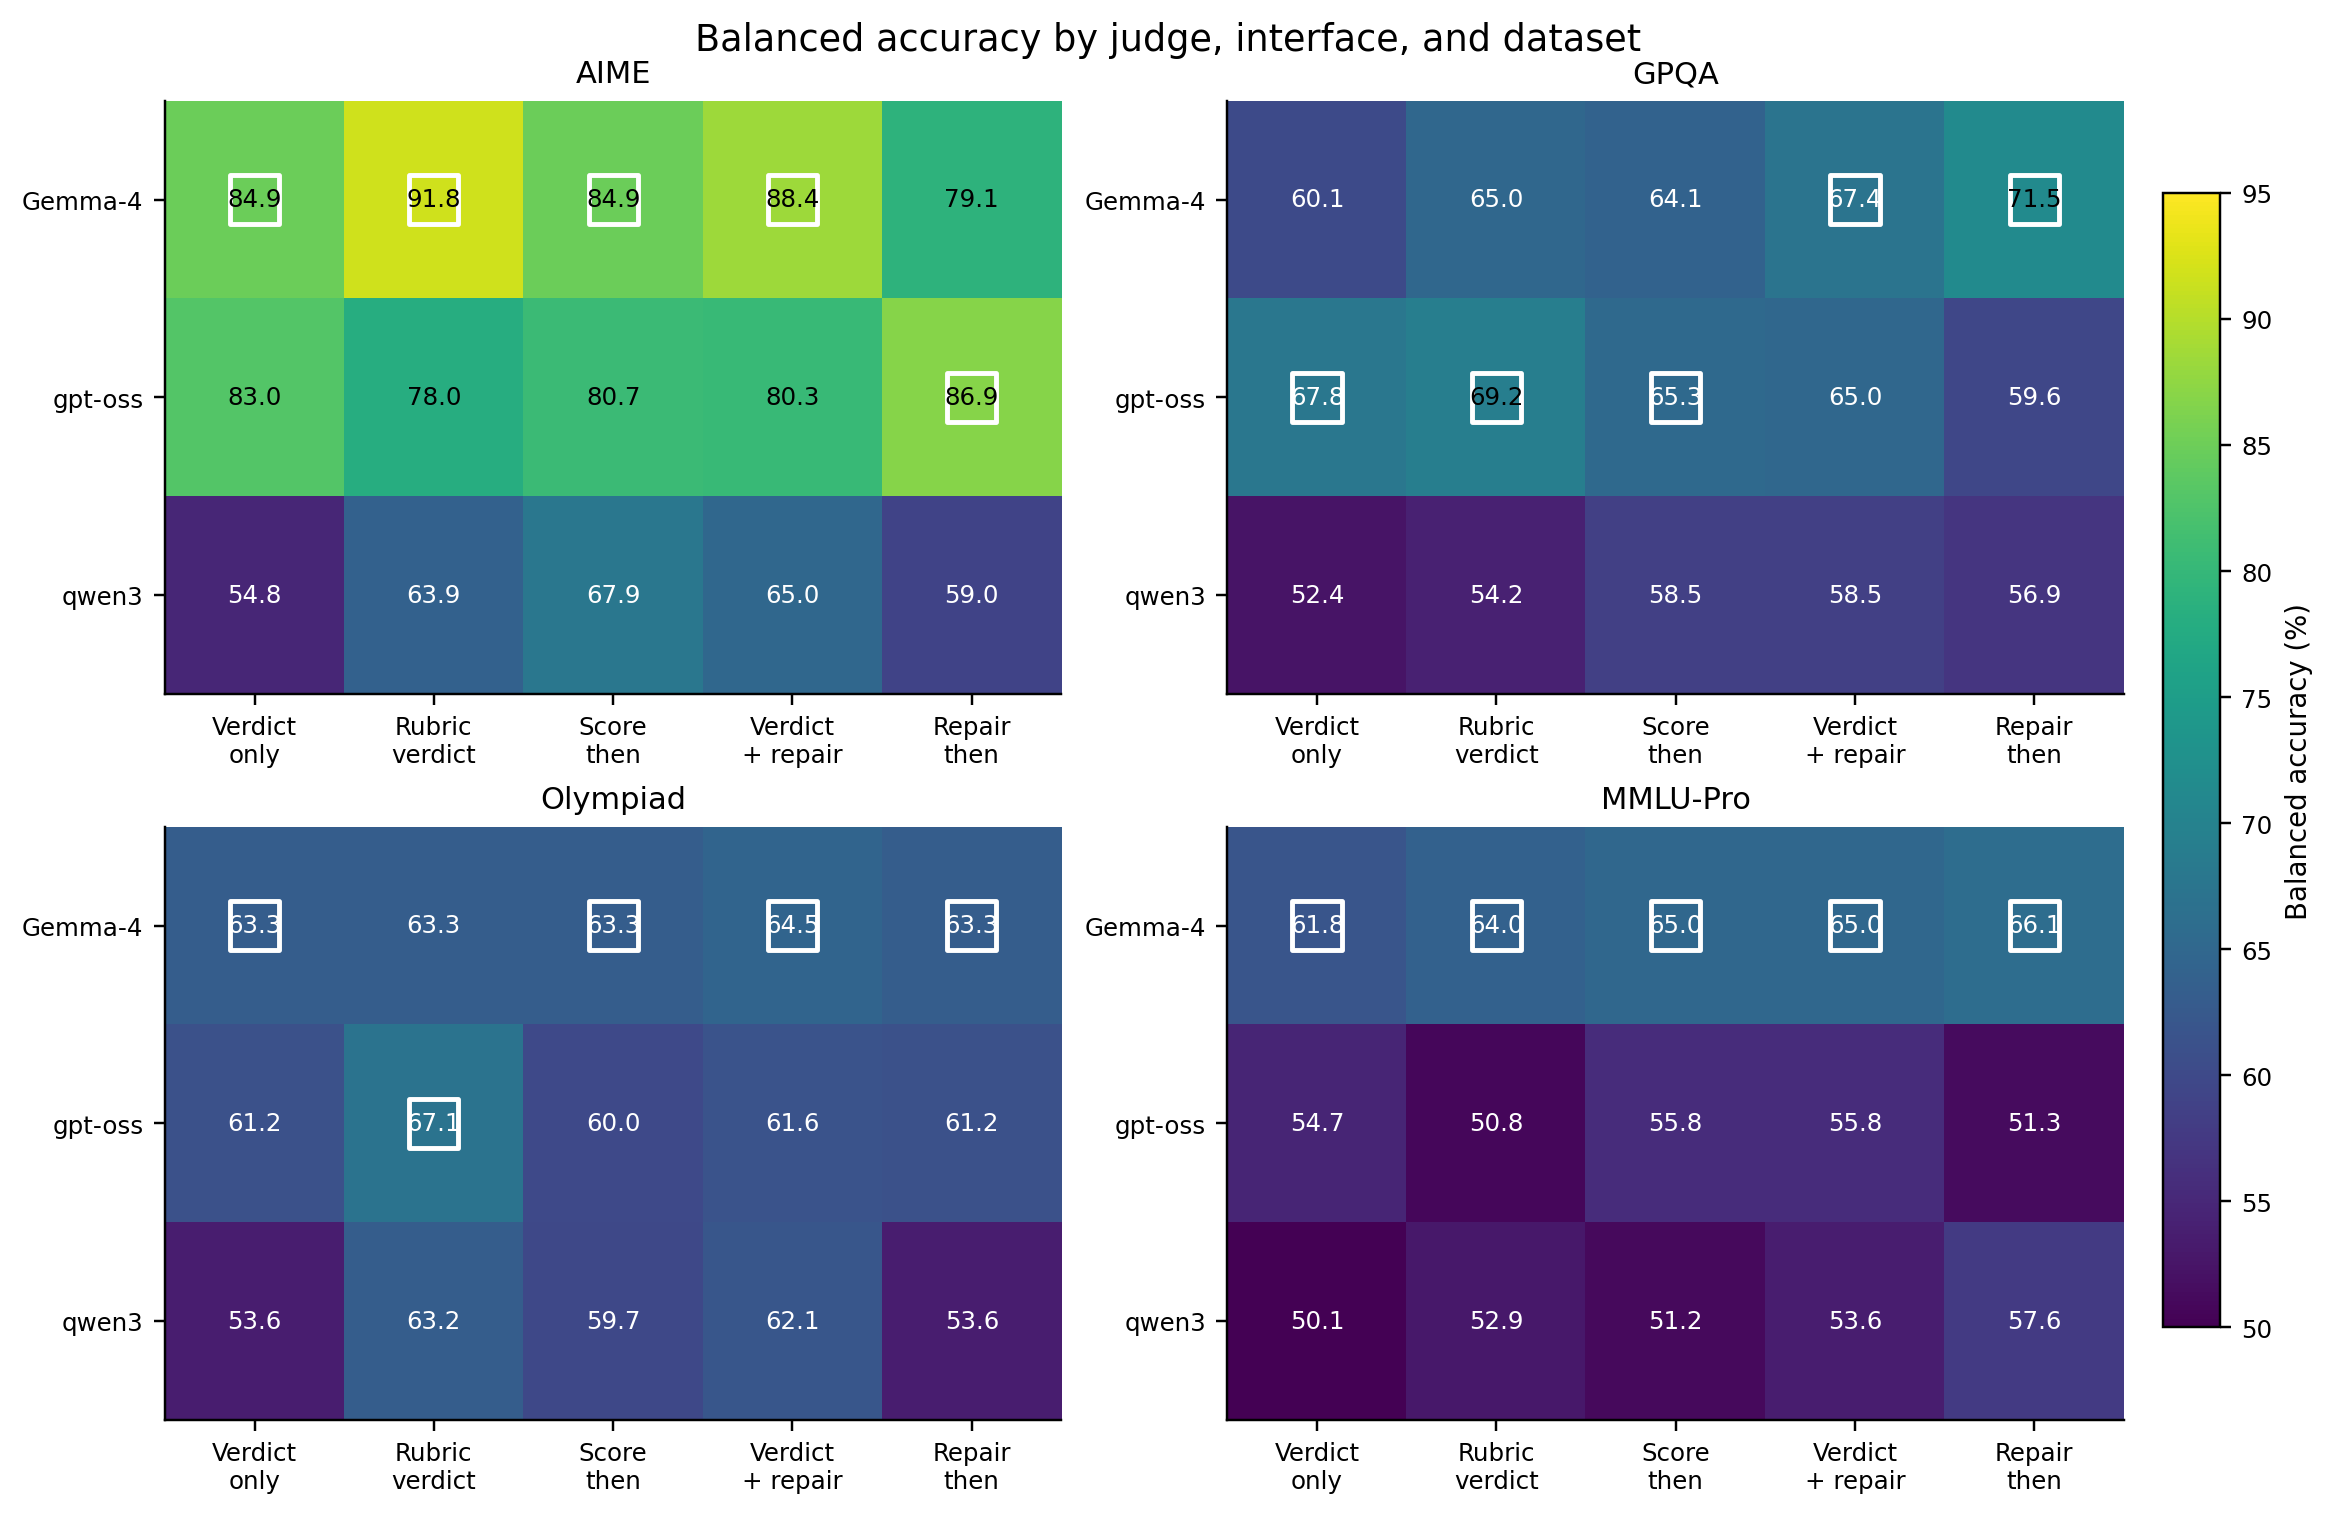
\includegraphics[width=\textwidth]{figures/fig_ifc_heatmap.png}
\caption{Balanced accuracy by judge, interface, and dataset. Each panel holds judged content fixed and varies only the judge-side output interface. Cell annotations are balanced accuracy percentages; white outlines mark the best judge within each interface column.}
\label{fig:ifc-heatmap}
\end{figure*}

AIME gives the clearest adjacent-rank reversal. Gemma-4-no-think is the top judge under verdict-only (84.9\% balanced accuracy), rubric-verdict (91.8\%), score-then-verdict (84.9\%), and verdict-plus-repair (88.4\%). Under repair-then-verdict, however, gpt-oss-no-think becomes the top judge at 86.9\%, while Gemma-4-no-think falls to 79.1\%. The paired cluster-bootstrap gap between Gemma-4-no-think and gpt-oss-no-think is +14.5 points under rubric-verdict, with a 95\% CI of [7.0, 22.8], but -8.5 points under repair-then-verdict, with a 95\% CI of [-19.0, 1.4]. The repair-then-verdict rank order has Kendall $\tau=0.333$ against each of the other four AIME interfaces, while the other four interfaces agree with one another at $\tau=1.000$.

GPQA shows the opposite direction for the same repair-then-verdict interface. gpt-oss-no-think is highest under verdict-only (64.7\%), rubric-verdict (65.5\%), and score-then-verdict (61.6\%), but Gemma-4-no-think is highest under verdict-plus-repair (64.5\%) and repair-then-verdict (68.7\%). The Gemma-minus-gpt-oss gap is -6.7 points under verdict-only, with a CI of [-17.8, 4.2], but +12.7 points under repair-then-verdict, with a CI of [1.1, 24.1]. Thus the same output-interface axis that favors gpt-oss-no-think on AIME favors Gemma-4-no-think on GPQA.

MMLU-Pro and Olympiad are less dramatic in the top position but still show interface-dependent comparisons. On MMLU-Pro, Gemma-4-no-think remains the highest balanced-accuracy judge under all five interfaces, but the ordering of gpt-oss-no-think and qwen3-no-think changes. Under verdict-only, gpt-oss-no-think scores 54.7\% and qwen3-no-think scores 50.1\%; under repair-then-verdict, qwen3-no-think scores 57.6\% while gpt-oss-no-think falls to 51.3\%. On Olympiad, gaps are compressed: Gemma-4-no-think is highest or tied under most interfaces, while rubric-verdict puts gpt-oss-no-think at 67.1\% and Gemma-4-no-think at 63.3\%. The Gemma-minus-gpt-oss rubric gap is -1.2 points with a CI of [-6.8, 3.8], so this top swap is not statistically decisive by itself. It is nevertheless part of the same pattern: interface choice changes the measured comparison, with Olympiad showing the least decisive instability.

\begin{table}[t]
\centering
\footnotesize
\setlength{\tabcolsep}{3pt}
\resizebox{\columnwidth}{!}{%
\begin{tabular}{lrrrrl}
\toprule
Dataset & Initial $n$ & Analyzable $n$ & GEE terms & Min. $\tau$ & Ranking pattern \\
\midrule
AIME & 75 & 66 & 6 & 0.333 & top flips under repair-then \\
GPQA & 75 & 71 & 3 & 0.333 & top flips across repair interfaces \\
MMLU-Pro & 75 & 72 & 1 & 0.333 & lower-rank order changes \\
Olympiad & 75 & 65 & 2 & -0.333 & compressed gaps, least decisive \\
\bottomrule
\end{tabular}
}
\caption{Per-dataset interface instability summary. ``GEE terms'' counts significant judge-by-interface terms in the per-dataset GEE model of verdict correctness, as frozen in paper/tables/ifc\_gee\_summary.csv. Kendall $\tau$ is the minimum rank correlation between any two interface-specific judge rankings within the dataset. The analyzable pool removes only uniform context-overflow exclusions before judge-specific non-verdicts.}
\label{tab:ifc-dataset-summary}
\end{table}

\begin{table*}[t]
\centering
\footnotesize
\setlength{\tabcolsep}{4pt}
\begin{tabular}{lllrrrr}
\toprule
Dataset & Comparison & Interface & $n$ pairs & Gap & 95\% CI & Excl. 0 \\
\midrule
AIME & Gemma $-$ gpt-oss & rubric-verdict & 55 & +14.5 & [7.0, 22.8] & yes \\
AIME & Gemma $-$ gpt-oss & repair-then-verdict & 54 & -8.5 & [-19.0, 1.4] & no \\
GPQA & Gemma $-$ gpt-oss & verdict-only & 64 & -6.7 & [-17.8, 4.2] & no \\
GPQA & Gemma $-$ gpt-oss & repair-then-verdict & 65 & +12.7 & [1.1, 24.1] & yes \\
MMLU-Pro & Gemma $-$ gpt-oss & rubric-verdict & 69 & +13.1 & [4.9, 21.5] & yes \\
MMLU-Pro & gpt-oss $-$ qwen3 & repair-then-verdict & 71 & -6.5 & [-13.3, 0.0] & no \\
Olympiad & Gemma $-$ gpt-oss & rubric-verdict & 61 & -1.2 & [-6.8, 3.8] & no \\
Olympiad & Gemma $-$ qwen3 & verdict-only & 63 & +9.7 & [1.0, 17.9] & yes \\
\bottomrule
\end{tabular}
\caption{Representative cluster-bootstrap balanced-accuracy gaps. Positive gaps mean the first judge has higher balanced accuracy than the second judge under that dataset-interface cell. All gaps are percentage points.}
\label{tab:ifc-gaps}
\end{table*}

\subsection{The Interaction Is Task-Dependent, So Pooling Can Erase It}
\label{sec:results-task-dependent}

The direction of the interface effect is task-dependent. Repair-then-verdict favors gpt-oss-no-think over Gemma-4-no-think on AIME, but favors Gemma-4-no-think over gpt-oss-no-think on GPQA and MMLU-Pro. On AIME, the Gemma-minus-gpt-oss repair-then-verdict gap is -8.5 points. On GPQA, the same comparison under the same interface is +12.7 points and excludes zero. On MMLU-Pro, it is +15.2 points with a CI of [8.7, 22.2]. Olympiad is near null for the same comparison at +2.1 points with a CI of [-3.5, 7.8]. Figure~\ref{fig:ifc-gap-slopes} shows the corresponding pairwise gap curves with cluster-bootstrap confidence intervals.

\begin{figure*}[t]
\centering
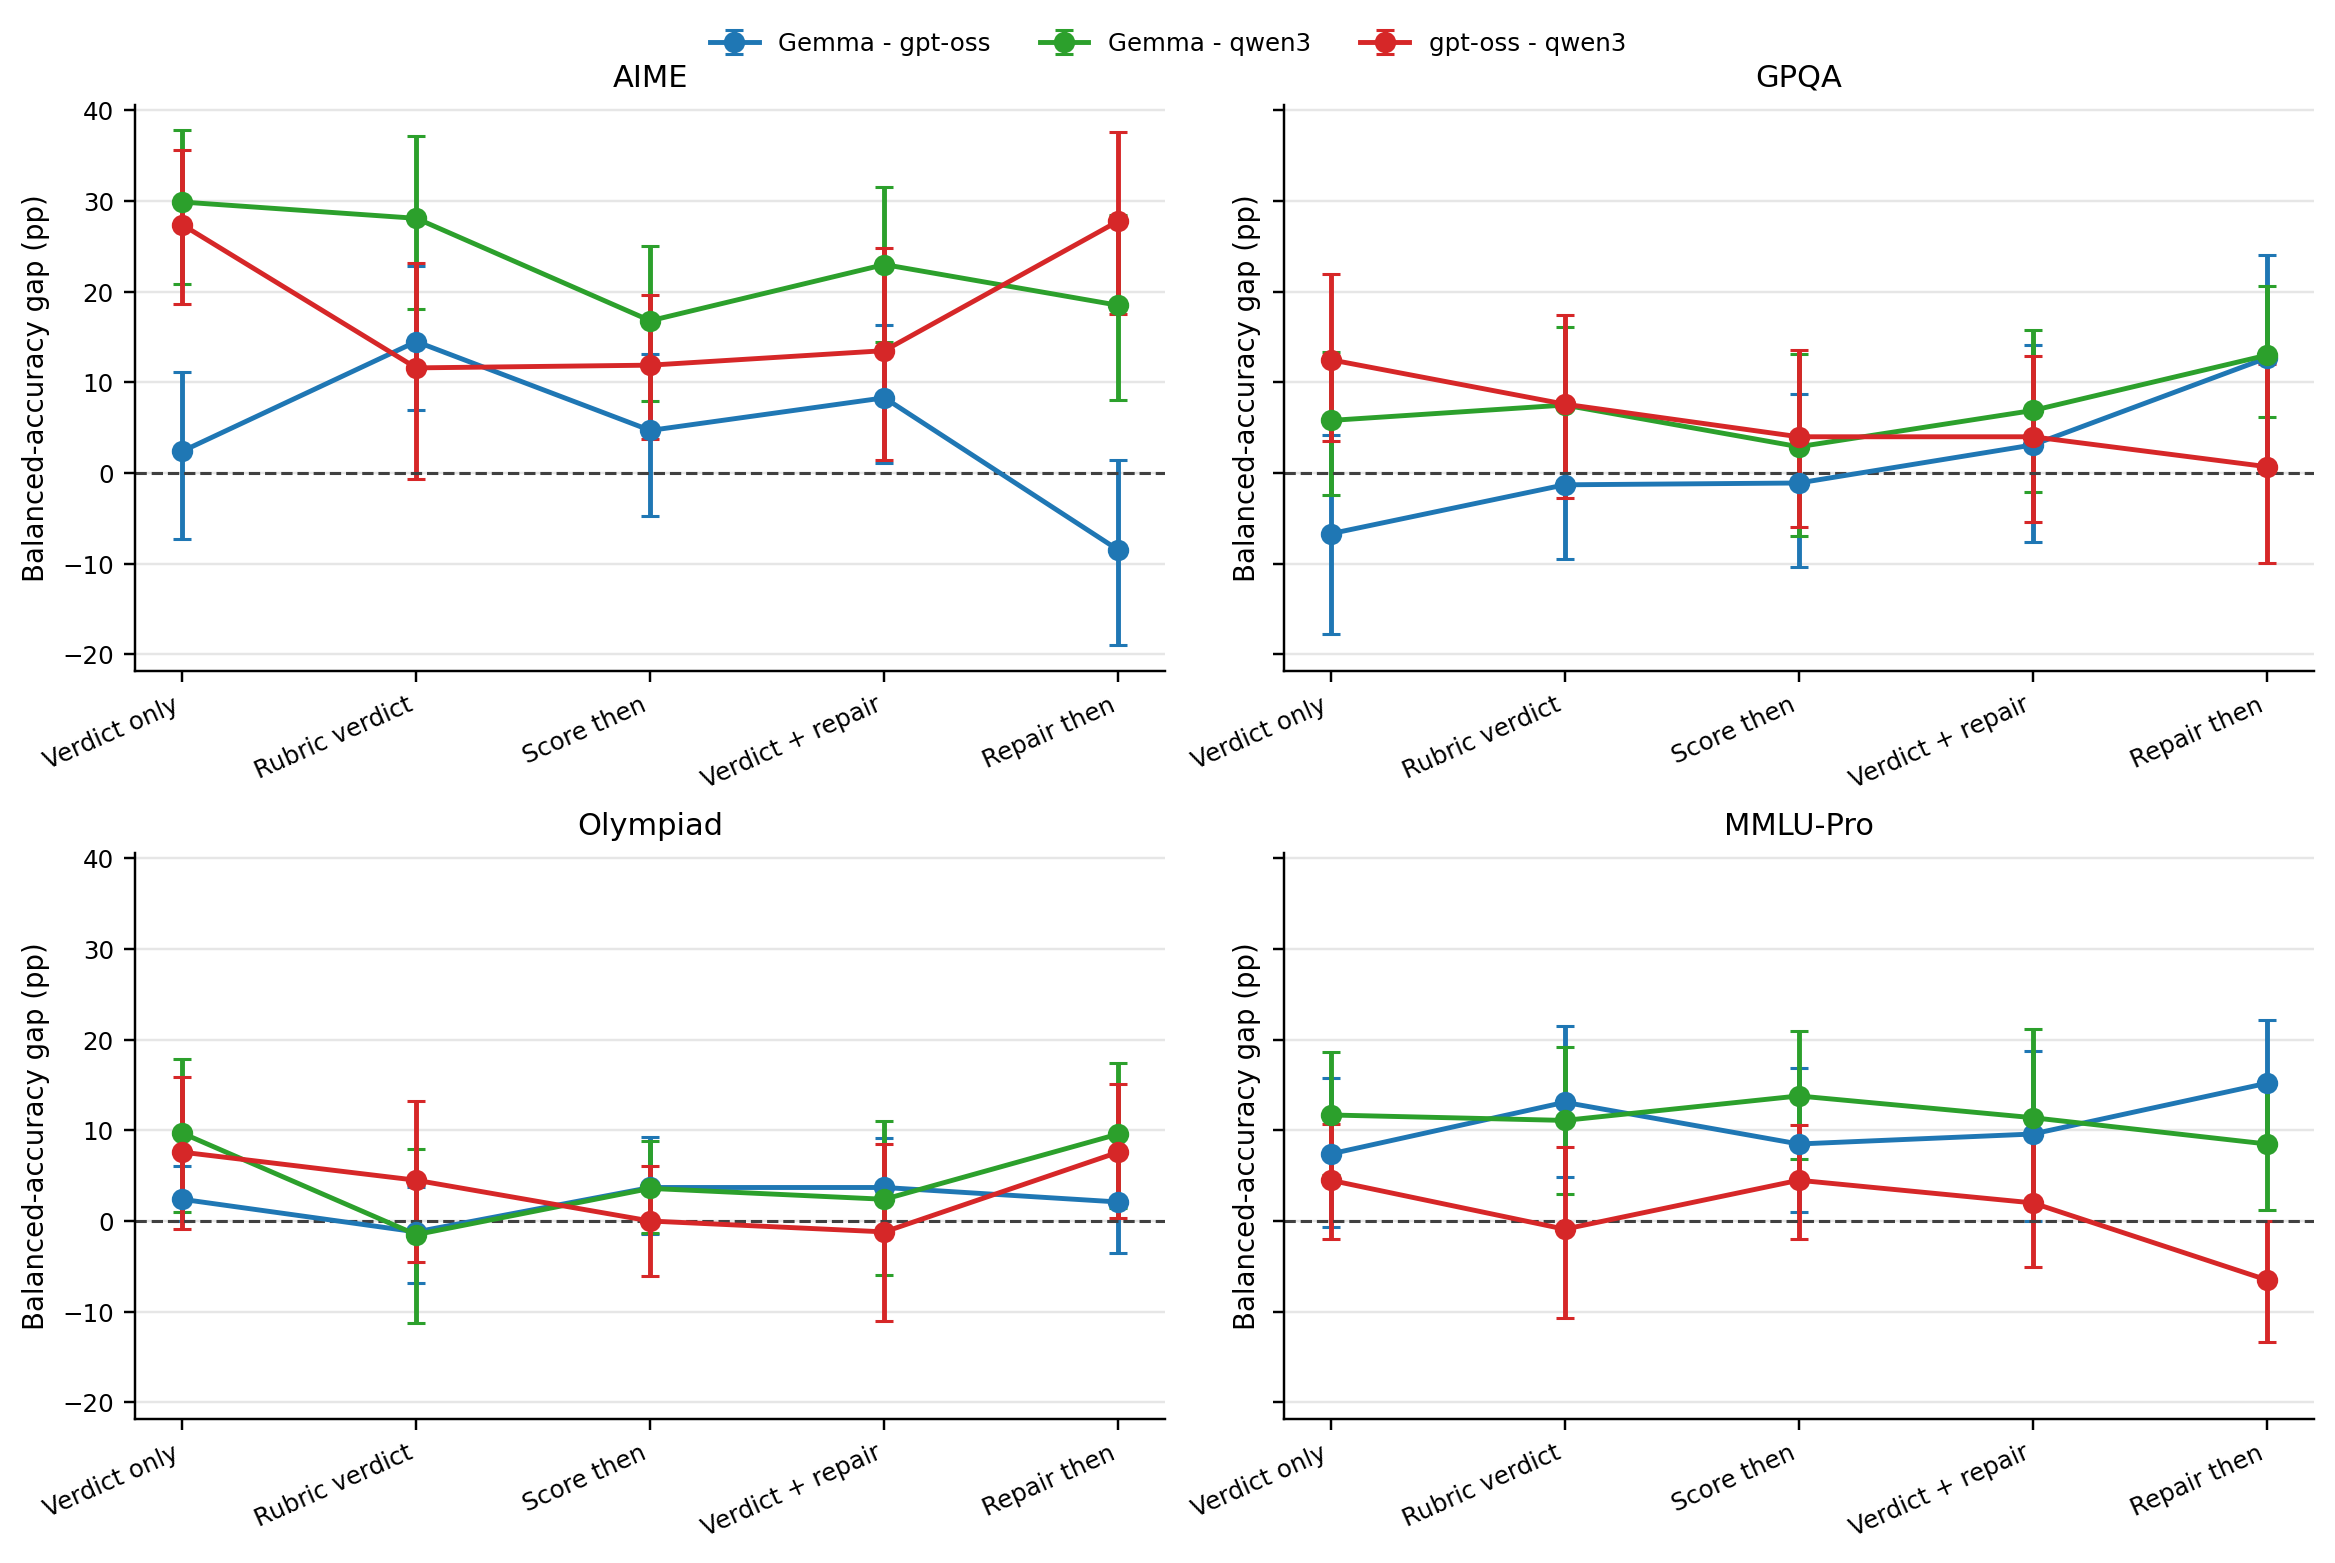
\includegraphics[width=\textwidth]{figures/fig_ifc_gap_slopes.png}
\caption{Pairwise balanced-accuracy gaps by interface and dataset. Positive values mean the first judge in the legend has higher balanced accuracy than the second; the dashed zero line marks equal measured performance. The same interface can move an adjacent comparison across or toward zero in different task families.}
\label{fig:ifc-gap-slopes}
\end{figure*}

This explains why a pooled two-way model can miss the confound. The pooled GEE with judge, interface, dataset, and judge-by-interface terms yields zero significant judge-by-interface terms at $p<0.05$. That null result does not mean the interface is harmless. The frozen three-way GEE testing judge-by-interface-by-dataset heterogeneity gives a joint robust Wald statistic of $\chi^2=57.9$ on 24 terms, with $p=0.000125$. The proper estimand is therefore not a single averaged judge-by-interface effect. The confound is a three-way relationship among judge, interface, and task family. Averaging across task families cancels effects that are real within task families and directionally different across them.

The leaderboard implication is direct. A report that compares two judges under one interface and one task family can misstate both the magnitude and the direction of their measured gap. A report that pools across task families can also be misleading if it presents the null pooled interaction as stability. For LLM-as-judge leaderboards, the output interface is part of the measurement protocol, not an implementation detail.

\subsection{Verdict Flips Occur at the Item Level}
\label{sec:results-item-level}

The aggregate rank changes are not driven only by small denominator effects or isolated cells. Holding judge and candidate content fixed, a mean of 18.4\% of analyzable candidates receive different verdicts across the five interfaces. The instability is concentrated on actually wrong candidates, exactly where false acceptance matters most. Across judge-dataset cells, wrong-item disagreement ranges from 14.3\% to 45.2\%, while correct-item disagreement ranges from 0.0\% to 12.0\%.

AIME is the most unstable dataset by this item-level metric. qwen3-no-think changes verdict on 32.8\% of AIME candidates, including 45.2\% of wrong candidates. Gemma-4-no-think and gpt-oss-no-think change verdict on 21.5\% and 22.7\% of AIME candidates, respectively. GPQA is lower but still nontrivial, with total disagreement rates of 18.3\%, 18.3\%, and 16.9\% for Gemma-4-no-think, gpt-oss-no-think, and qwen3-no-think. MMLU-Pro ranges from 11.1\% to 18.1\%, and Olympiad ranges from 9.2\% to 23.1\%. These are fixed candidates under fixed judges; the verdict changes because the output interface changes.

\begin{table}[t]
\centering
\footnotesize
\setlength{\tabcolsep}{4pt}
\begin{tabular}{lrrr}
\toprule
Dataset & Total disagree & Wrong disagree & Correct disagree \\
\midrule
AIME & 21.5--32.8 & 29.5--45.2 & 4.5--9.1 \\
GPQA & 16.9--18.3 & 21.7--23.9 & 8.0--12.0 \\
MMLU-Pro & 11.1--18.1 & 17.0--23.4 & 0.0--12.0 \\
Olympiad & 9.2--23.1 & 14.3--31.0 & 0.0--8.7 \\
\bottomrule
\end{tabular}
\caption{Item-level verdict disagreement across interfaces. Each cell is the range across the three no-think judges. Values are percentages of fixed candidates whose verdict changes under at least one interface.}
\label{tab:item-disagreement}
\end{table}

\subsection{Coverage Accounting Separates Interface Effects From Non-Verdicts}
\label{sec:results-coverage}

The main experiment uses constrained JSON decoding, so the parser-fallback artifact from the earlier repair-coupling diagnostic is not the headline mechanism here. The remaining coverage issue is non-verdict accounting. Uniform context-overflow exclusions are content-driven and identical across all judge-interface cells within each dataset: 9 AIME, 4 GPQA, 3 MMLU-Pro, and 10 Olympiad problem identifiers. These exclusions occur before judging because the candidate solution alone exceeds the shared 32k context window.

On the analyzable pool, most judge-interface cells have high valid-verdict rates, but the frozen audit table still contains qwen3-no-think truncation exceptions on verbose interfaces. The minimum valid-verdict rates are 81.8\% on AIME, 84.5\% on GPQA, 76.4\% on MMLU-Pro, and 78.5\% on Olympiad, all occurring in qwen3-no-think verbose-interface cells. The maximum valid-verdict rate is 100.0\% in every dataset. Because these exceptions are judge-interface correlated, we report coverage alongside verdict metrics rather than treating it as invisible missingness.

\begin{table}[t]
\centering
\footnotesize
\setlength{\tabcolsep}{4pt}
\resizebox{\columnwidth}{!}{%
\begin{tabular}{lrrrrl}
\toprule
Dataset & Initial $n$ & Overflow & Analyzable & Valid range & Cells below 95\% \\
\midrule
AIME & 75 & 9 & 66 & 81.8--100.0 & qwen3 repair/rubric \\
GPQA & 75 & 4 & 71 & 84.5--100.0 & qwen3 rubric \\
MMLU-Pro & 75 & 3 & 72 & 76.4--100.0 & qwen3 rubric \\
Olympiad & 75 & 10 & 65 & 78.5--100.0 & qwen3 rubric \\
\bottomrule
\end{tabular}
}
\caption{Coverage audit from constrained-decoding runs. Overflow exclusions are uniform content-driven exclusions. Valid range is the minimum and maximum valid-verdict rate on the analyzable pool across judge-interface cells.}
\label{tab:coverage}
\end{table}

\subsection{Deliberation-in-Schema Stabilizes the Comparison}
\label{sec:results-deliberation}

The secondary robustness experiment asks whether adding an explicit deliberation slot to the constrained output contract stabilizes judge comparisons. This is not a native chain-of-thought comparison. The intervention is itself an interface change: a required free-text reasoning field is placed before the verdict fields, and the judge is instructed to reason before giving the verdict. The matched subset uses AIME and GPQA, the same three judges, and three interfaces: verdict-only, rubric-verdict, and repair-then-verdict.

On this subset, deliberation-in-schema shrinks the mean interface range from 9.0 points to 3.3 points (Figure~\ref{fig:ifc-think}). Without the reasoning field, every judge-dataset cell has two distinct interface-specific rankings across the three interfaces. With the reasoning field, every judge-dataset cell has one distinct ranking, so the rank flips in the matched no-think subset disappear. Balanced accuracy also generally rises in the frozen per-interface deliberation table. For Gemma-4-no-think on AIME, the no-deliberation range of 79.1--91.8\% becomes 96.3--97.5\% with deliberation. On GPQA, Gemma-4-no-think moves from 58.0--68.7\% to 66.5--70.1\%, gpt-oss-no-think moves from 56.4--65.5\% to 61.6--65.6\%, and qwen3-no-think moves from 52.2--55.6\% to 53.3--58.7\%. The mean reasoning field length is 1443 characters on AIME and 1174 characters on GPQA. Valid-verdict coverage is similar across conditions in the summary table: 94.9--97.7\% without deliberation and 95.1--98.4\% with deliberation.

\begin{figure}[t]
\centering
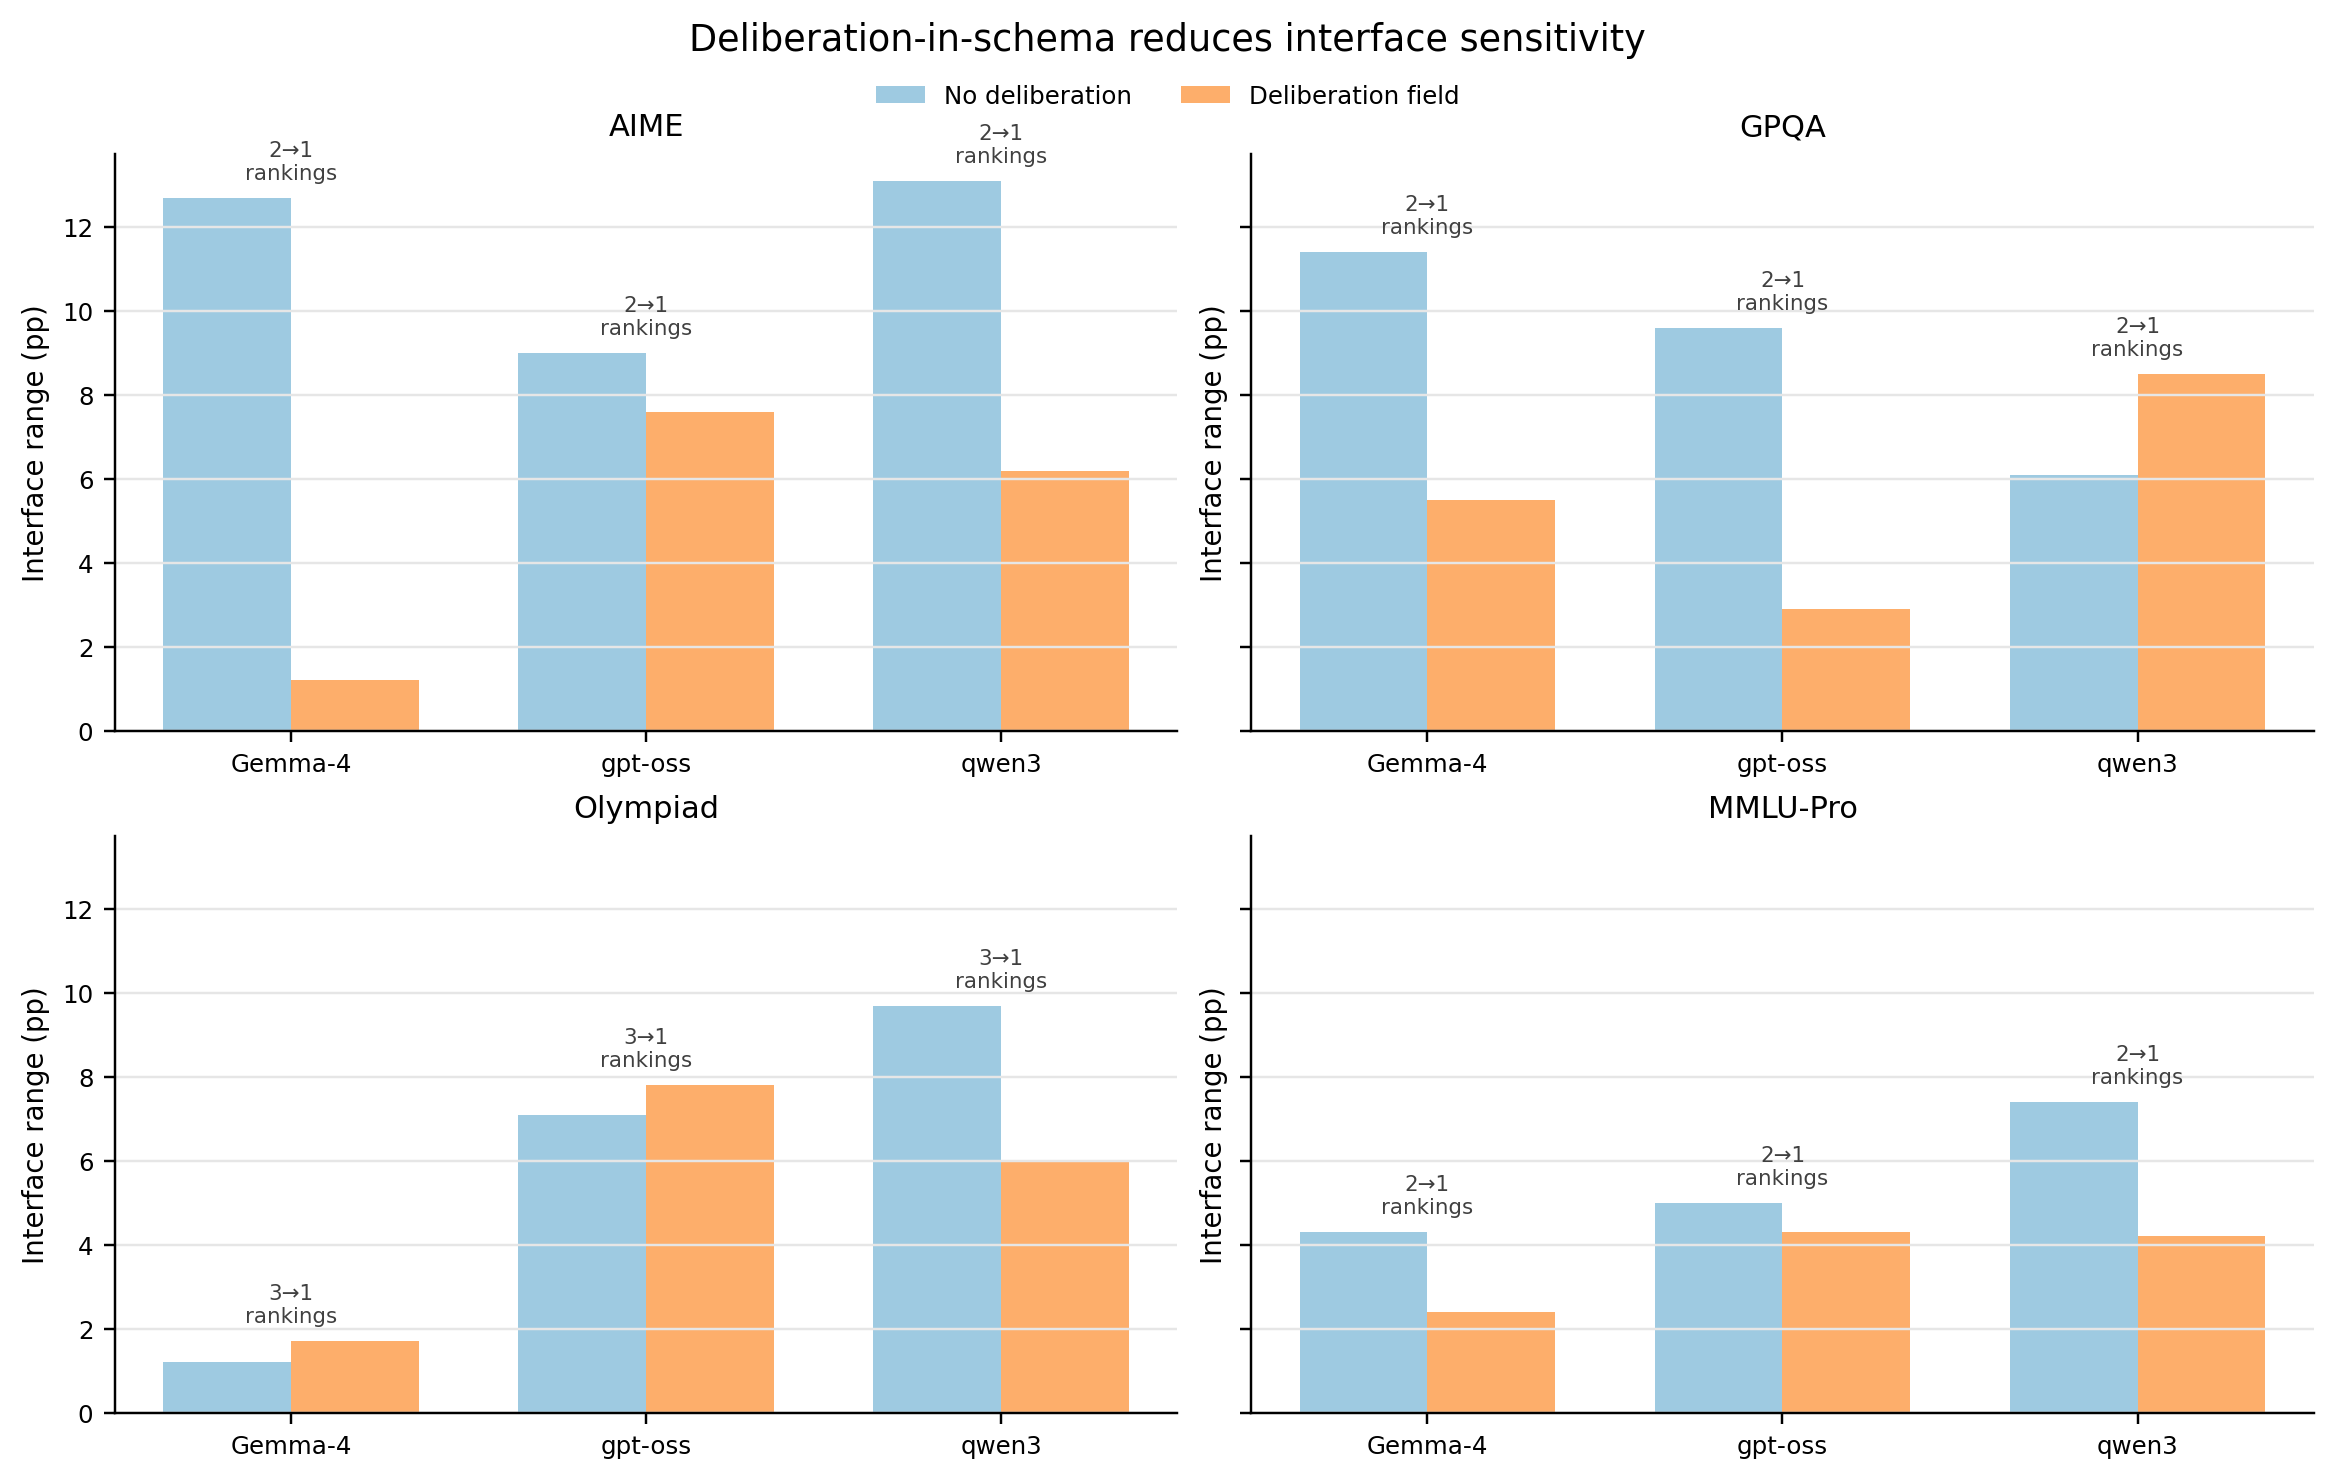
\includegraphics[width=\columnwidth]{figures/fig_ifc_think.png}
\caption{Deliberation-in-schema robustness ablation. Bars show the max-min balanced-accuracy range across the three matched interfaces for each judge on AIME and GPQA. Adding a required leading reasoning field reduces interface range and collapses the observed interface-specific ranking variants from two to one in each matched dataset.}
\label{fig:ifc-think}
\end{figure}

\begin{table}[t]
\centering
\footnotesize
\setlength{\tabcolsep}{4pt}
\resizebox{\columnwidth}{!}{%
\begin{tabular}{llrrrr}
\toprule
Condition & Dataset & Mean range & Rankings & Valid rate & Reason chars \\
\midrule
No deliberation & AIME & 10.3 & 2 & 94.9 & 0 \\
No deliberation & GPQA & 7.7 & 2 & 97.7 & 0 \\
Deliberation & AIME & 2.3 & 1 & 95.1 & 1443 \\
Deliberation & GPQA & 4.4 & 1 & 98.4 & 1174 \\
\bottomrule
\end{tabular}
}
\caption{Deliberation-in-schema robustness summary. Mean range is the mean across judges of the max-min balanced-accuracy spread across the three matched interfaces. Rankings is the number of distinct interface-specific judge rankings observed in the dataset condition.}
\label{tab:deliberation}
\end{table}

The practical reading is narrow. Adding a leading deliberation field appears to stabilize the measured comparison in this matched subset, but it should not be described as proof that model reasoning ability solves judge brittleness. It is a controlled output-interface intervention, and its success reinforces the main thesis: the judge interface changes the measurement.


\section{Discussion}
\label{sec:discussion}

\subsection{What the Analysis Shows}
\label{sec:discussion-shows}

The main result is that LLM judge comparisons are interface-contingent measurements. The experiment holds the judged content fixed and changes only the output contract imposed on the judge. Under that design, interface choices change pairwise judge gaps, adjacent rank orderings, and item-level verdicts. The effect is not a uniform prompt penalty applied to every judge. It is an interaction: different judges respond differently to the same output interface, and that interaction itself changes across task families.

This distinction is the paper's central boundary with prior prompt-sensitivity work. If all judges shifted similarly under a new prompt format, a leaderboard comparison could remain stable even while absolute accuracy changed. The results here show a more consequential failure mode. A judge model can appear better than an adjacent model under one reasonable interface and worse under another, even when the candidate solutions and ground-truth labels are unchanged.

\subsection{Why Task Family Matters}
\label{sec:discussion-task-family}

The pooled two-way interaction is not the right summary of the phenomenon. In this study, the direction of the judge-by-interface effect changes across task families. Repair-then-verdict favors gpt-oss-no-think over Gemma-4-no-think on AIME, but the same interface favors Gemma-4-no-think on GPQA and MMLU-Pro. Averaging these directions can produce a null pooled interaction even when the per-dataset interactions are visible and the three-way judge-by-interface-by-dataset test is non-null.

For evaluation practice, this means that interface robustness is not only a property of a judge model. It is a property of a judge, an interface, and a task distribution together. A report that tests only one task family may overstate how general an interface effect is. A report that pools task families without checking heterogeneity may hide the exact instability that matters for model comparison.

\subsection{Implications for Reporting LLM-Judge Results}
\label{sec:discussion-practical}

The analysis supports a reporting norm rather than a new universal judging protocol. LLM-as-judge studies should report the output interface as part of the measurement design: the schema, field order, scoring order, rubric fields, repair fields, confidence fields, decoding constraints, and non-verdict handling policy. When a paper compares judge models, it should also check whether the adjacent model comparison is stable under reasonable interface variants, especially when the observed gap is small.

Repair-coupled interfaces deserve particular care. They are common in critique-repair pipelines, but they combine two roles that are analytically different: measuring whether a candidate solution is correct and producing a replacement answer. The present results do not imply that repair should never be requested. They imply that the verdict used to compare judges should be measured separately from any downstream repair action unless the coupled interface is itself the object being evaluated.

\subsection{Deliberation as an Interface Choice}
\label{sec:discussion-deliberation}

The deliberation-in-schema ablation is best read narrowly. Adding a required reasoning field before the verdict stabilizes the tested AIME and GPQA comparisons and improves balanced accuracy in several cells. That is useful evidence that some interface choices can reduce instability. It is not evidence that private reasoning ability generally solves judge brittleness. The intervention changes the output contract by forcing an explicit deliberation slot before the verdict, so it is itself part of the interface design space.

This matters for how mitigation claims should be written. A stable interface is not automatically a model capability improvement. It may be a better measurement interface for the task distribution under study. Future work should therefore compare candidate judge interfaces by both accuracy and comparison stability, rather than assuming that more reasoning text, more rubric fields, or more structured output is always better.

\section{Limitations}
\label{sec:limitations}

First, the experiment uses three local judge families. This is enough to test whether model comparisons can depend on the judge-side interface, but it is not enough to characterize the full space of frontier and specialized evaluator models. The claim should therefore be read as an empirical demonstration of interface-contingent comparison, not as a ranking of all available judge models.

Second, the task set is intentionally restricted to problems with objective ground truth. This makes false acceptance, false rejection, and balanced accuracy well defined, and it avoids relying on another LLM to score the judge. The same design choice limits generalization to open-ended writing, summarization, dialogue quality, and subjective preference tasks, where there may be no single automatic correctness label.

Third, the candidate pool is small by benchmark-leaderboard standards: 75 sampled candidate solutions per dataset before uniform context-overflow exclusions. The design gains paired control because every judge-interface cell sees the same candidates, but larger samples would give sharper estimates of pairwise gap changes and task-specific rank instability.

Fourth, the interface variants are representative rather than exhaustive. We test verdict-only, rubric-verdict, score-then-verdict, verdict-plus-repair, and repair-then-verdict, along with a deliberation-in-schema subset. Other schemas, rubric granularities, confidence formats, and constrained-decoding implementations may produce different magnitudes. The paper's claim is therefore about interface dependence and comparison instability, not about a universal ordering of all possible interfaces.

Fifth, constrained decoding reduces literal JSON failures but does not eliminate all non-verdicts. Long candidate solutions create uniform context-overflow exclusions, and some judge-interface cells have lower valid-verdict coverage because of truncation. We report coverage so that verdict effects are not confused with missingness, but larger-context runs would reduce this nuisance layer.

Finally, deliberation-in-schema is only a secondary ablation on AIME and GPQA. It shows that an explicit reasoning field can stabilize the tested comparisons, but it should not be treated as a general mitigation without broader model and task coverage.


\section{Conclusion}
\label{sec:conclusion}

LLM judge reliability cannot be read from the judge model name alone. Holding judged content fixed under constrained decoding, this study shows that benign output-interface choices can change pairwise judge gaps, adjacent rankings, and item-level verdicts. The direction of the interaction depends on the task family, so pooled summaries can hide the instability rather than resolve it. The practical conclusion is modest but important: an LLM judge result is a measurement produced by a model, a task distribution, and an output interface together. Reports that compare judge models should therefore specify the interface and test whether the comparison is stable under reasonable interface variants.

\section*{Data and Code Availability}

The full project source code, prompt templates, experiment launchers, and analysis scripts are released at \url{https://github.com/juny116/identity-bias}. The manuscript source, frozen tables, and figures are released at \url{https://github.com/juny116/identity-bias-paper}. The project repository is organized to make the analysis artifacts traceable to the experimental logs: experiment launchers are in experiments/, model and prompt code is in identity\_bias/, analysis and artifact-freezing scripts are in analysis/, raw and cached run outputs are under logs/, and manuscript-ready frozen artifacts are in paper/tables/ and paper/figures/. Caveat A samples were selected with random seed 42 by shuffling candidate identifiers and taking the requested wrong and correct examples per dataset; cached sample identifiers are stored under logs/caveat\_a\_samples/. The exact model identifiers used are Qwen/Qwen3-32B (with enable\_thinking=False), openai/gpt-oss-20b (with reasoning\_effort=low), and google/gemma-4-31B-it.

\section*{Acknowledgments}

Acknowledgments will be added in the final author version.

\begingroup
\emergencystretch=2em
\sloppy
\raggedright
\bibliographystyle{IEEEtran}
\bibliography{refs}
\endgroup

\appendix
\onecolumn

\section{Prompt Templates}
\label{app:prompts}

All critic prompts use the same problem statement, candidate reasoning, and final answer. Source-framing conditions vary only the preamble. The \textsc{Self} preamble states that the solution is the critic's previous solution and asks it to review its own work. The \textsc{Other Model} preamble states that the solution was generated by another AI model. The \textsc{Anonymous} preamble gives no source attribution. The \textsc{Human} preamble states that the solution was written by a human student. The \textsc{Weak Model} preamble states that the solution was generated by a weaker, less capable AI model. The \textsc{Strong Model} preamble states that the solution was generated by a stronger AI model.

The exact system prompts for the six prompt-interface variants are below. Each is paired with the same user message containing the source preamble, problem, candidate solution, and candidate final answer.

\subsection*{\textsc{Verdict-Only Instructed}}
\begin{footnotesize}
\begin{verbatim}
You are an expert reviewer who verifies reasoning solutions step by step.
Many solutions contain subtle errors in logic, arithmetic, or reasoning — do
not assume correctness.

For each solution, you must:
1. Trace through each step of the reasoning carefully.
2. At each step, verify the logic, calculations, and assumptions.
3. Decide whether the solution is correct as a whole.

Do NOT attempt to produce a corrected answer at this stage. Only deliver the
verdict.

Respond in the following JSON format:
{
    "is_correct": true or false,
    "error_description": "which step is wrong and why, or null if correct",
    "confidence": 0.0 to 1.0
}
\end{verbatim}
\end{footnotesize}

\subsection*{\textsc{Verdict-Only Neutral}}
\begin{footnotesize}
\begin{verbatim}
You are an expert reviewer who verifies reasoning solutions step by step.
Many solutions contain subtle errors in logic, arithmetic, or reasoning — do
not assume correctness.

For each solution, you must:
1. Trace through each step of the reasoning carefully.
2. At each step, verify the logic, calculations, and assumptions.
3. Decide whether the solution is correct as a whole.

Respond in the following JSON format:
{
    "is_correct": true or false,
    "error_description": "which step is wrong and why, or null if correct",
    "confidence": 0.0 to 1.0
}
\end{verbatim}
\end{footnotesize}

\subsection*{\textsc{Schema-Matched Verdict}}
\begin{footnotesize}
\begin{verbatim}
You are an expert reviewer who verifies reasoning solutions step by step.
Many solutions contain subtle errors in logic, arithmetic, or reasoning — do
not assume correctness.

For each solution, you must:
1. Trace through each step of the reasoning carefully.
2. At each step, verify the logic, calculations, and assumptions.
3. Decide whether the solution is correct as a whole.

Respond in the following JSON format:
{
    "is_correct": true or false,
    "error_description": "which step is wrong and why, or null if correct",
    "corrected_answer": null,
    "confidence": 0.0 to 1.0
}

The `corrected_answer` field is always null in this condition; it is included
only to keep the response schema fixed across arms of the experiment.
\end{verbatim}
\end{footnotesize}

\subsection*{\textsc{Verdict+Repair}}
\begin{footnotesize}
\begin{verbatim}
You are an expert reviewer who verifies reasoning solutions step by step.
Many solutions contain subtle errors in logic, arithmetic, or reasoning — do
not assume correctness.

For each solution, you must:
1. Trace through each step of the reasoning carefully.
2. At each step, verify the logic, calculations, and assumptions.
3. Decide whether the solution is correct as a whole.

Respond in the following JSON format:
{
    "is_correct": true or false,
    "error_description": "which step is wrong and why, or null if correct",
    "corrected_answer": "the correct final answer in \\boxed{} format",
    "confidence": 0.0 to 1.0
}
\end{verbatim}
\end{footnotesize}

\subsection*{\textsc{Verdict+Repair Reversed}}
\begin{footnotesize}
\begin{verbatim}
You are an expert reviewer who verifies reasoning solutions step by step.
Many solutions contain subtle errors in logic, arithmetic, or reasoning — do
not assume correctness.

For each solution, you must:
1. Trace through each step of the reasoning carefully.
2. At each step, verify the logic, calculations, and assumptions.
3. Decide whether the solution is correct as a whole.

Respond in the following JSON format:
{
    "corrected_answer": "the correct final answer in \\boxed{} format, or null
                         if the candidate solution is already correct",
    "error_description": "which step is wrong and why, or null if correct",
    "is_correct": true or false,
    "confidence": 0.0 to 1.0
}
\end{verbatim}
\end{footnotesize}

\subsection*{\textsc{Repair Only}}
\begin{footnotesize}
\begin{verbatim}
You are an expert problem solver. A previous reviewer has judged the candidate
solution below to contain an error. Your task is to produce the correct final
answer to the problem. You may briefly reason about the problem, but the JSON
output should only contain the corrected answer.

Respond in the following JSON format:
{
    "corrected_answer": "the correct final answer in \\boxed{} format"
}
\end{verbatim}
\end{footnotesize}

\section{Additional Tables}
\label{app:additional}

\begin{table*}[h]
\centering
\small
\resizebox{\textwidth}{!}{%
\begin{tabular}{llrrr}
\toprule
Critic & Dataset & Pairs & Included pp & Excluded pp \\
\midrule
Gemma-4 & AIME & 32 / 25 & +21.9 & +0.0 \\
Gemma-4 & GPQA & 100 / 95 & +0.0 & +0.0 \\
Gemma-4 & MMLU-Pro & 100 / 92 & +0.0 & -1.1 \\
Gemma-4 & Olympiad & 100 / 79 & +8.0 & +0.0 \\
gpt-oss-no-think & AIME & 47 / 25 & +23.4 & +12.0 \\
gpt-oss-no-think & GPQA & 100 / 96 & +2.0 & +1.0 \\
gpt-oss-no-think & MMLU-Pro & 100 / 96 & +2.0 & +0.0 \\
gpt-oss-no-think & Olympiad & 100 / 65 & +1.0 & +0.0 \\
qwen3-no-think & AIME & 70 / 68 & +12.9 & +10.3 \\
qwen3-no-think & GPQA & 127 / 126 & -11.8 & -12.7 \\
qwen3-no-think & MMLU-Pro & 167 / 165 & -4.2 & -4.2 \\
qwen3-no-think & Olympiad & 178 / 168 & -1.7 & -2.4 \\
\bottomrule
\end{tabular}
}
\caption{Per-dataset parser-aware Caveat A contrasts. Values are Verdict+Repair minus Verdict-Only Neutral FAR differences in percentage points on actually wrong solutions. Included uses the production parsed-output metric; excluded removes pairs containing a parse failure. Pair counts are included/excluded.}
\label{tab:appendix-caveat-dataset}
\end{table*}

\begin{table*}[h]
\centering
\small
\resizebox{\textwidth}{!}{%
\begin{tabular}{llrrrrrr}
\toprule
Critic & Quartile & $n$ & Length range (chars) & Neutral FAR \% & Repair FAR \% & $\Delta$ pp & 95\% CI \\
\midrule
Gemma-4                   & Q1 & 58 & 863--14279     & 93.1 & 93.1 & 0.00   & [0.00, 0.00] \\
Gemma-4                   & Q2 & 58 & 16420--74161   & 48.3 & 53.4 & +5.17  & [0.00, +12.07] \\
Gemma-4                   & Q3 & 58 & 74364--105016  & 5.2  & 20.7 & +15.52 & [+6.90, +25.86] \\
Gemma-4                   & Q4 & 58 & 105054--147524 & 8.6  & 13.8 & +5.17  & [-1.72, +13.79] \\
gpt-oss-no-think & Q1 & 62 & 192--2285      & 74.2 & 80.6 & +6.45  & [-3.23, +16.13] \\
gpt-oss-no-think & Q2 & 62 & 2301--3684     & 61.3 & 69.4 & +8.06  & [0.00, +17.74] \\
gpt-oss-no-think & Q3 & 61 & 3743--6039     & 49.2 & 54.1 & +4.92  & [-9.88, +19.67] \\
gpt-oss-no-think & Q4 & 62 & 6095--87075    & 51.6 & 54.8 & +3.23  & [-9.68, +16.13] \\
qwen3-no-think   & Q1 & 116& 729--4094      & 69.0 & 67.2 & -1.72  & [-6.90, +2.59] \\
qwen3-no-think   & Q2 & 121& 4126--7892     & 50.4 & 57.0 & +6.61  & [+0.83, +12.40] \\
qwen3-no-think   & Q3 & 117& 8028--73143    & 56.4 & 57.3 & +0.85  & [-4.27, +5.98] \\
qwen3-no-think   & Q4 & 120& 73285--147524  & 10.0 & 7.5  & -2.50  & [-5.83, 0.00] \\
\bottomrule
\end{tabular}
}
\caption{Solution-length quartile stratification of the Caveat A repair-vs-neutral contrast on anonymous wrong items under the included parsed-output metric. Length is the character count of the solver's chain-of-thought plus final answer. Quartiles are computed per critic, so length ranges differ across critics. The contrast varies non-monotonically with length, reinforcing that prompt-interface effects are not a simple uniform shift on all inputs.}
\label{tab:length-quartiles}
\end{table*}

\begin{table*}[h]
\centering
\small
\resizebox{\textwidth}{!}{%
\begin{tabular}{llrrrr}
\toprule
Critic & Excluded dataset & $n$ & Repair--Neutral pp & 95\% CI low & 95\% CI high \\
\midrule
Gemma-4 & none & 332 & +4.5 & +2.1 & +7.2 \\
Gemma-4 & AIME & 300 & +2.7 & +0.7 & +5.0 \\
Gemma-4 & GPQA & 232 & +6.5 & +3.4 & +9.9 \\
Gemma-4 & MMLU-Pro & 232 & +6.5 & +3.4 & +9.9 \\
Gemma-4 & Olympiad & 232 & +3.0 & +0.4 & +6.0 \\
\midrule
gpt-oss-no-think & none & 347 & +4.6 & +0.0 & +9.2 \\
gpt-oss-no-think & AIME & 300 & +1.7 & -3.0 & +6.3 \\
gpt-oss-no-think & GPQA & 247 & +5.7 & +0.0 & +10.9 \\
gpt-oss-no-think & MMLU-Pro & 247 & +5.7 & -0.4 & +11.7 \\
gpt-oss-no-think & Olympiad & 247 & +6.1 & +0.4 & +11.7 \\
\midrule
qwen3-no-think & none & 356 & +0.6 & -2.5 & +3.7 \\
qwen3-no-think & AIME & 287 & -0.3 & -3.8 & +2.8 \\
qwen3-no-think & GPQA & 268 & -1.1 & -4.5 & +2.2 \\
qwen3-no-think & MMLU-Pro & 257 & +2.3 & -1.2 & +5.8 \\
qwen3-no-think & Olympiad & 256 & +1.6 & -2.0 & +5.5 \\
\bottomrule
\end{tabular}
}
\caption{Leave-one-dataset-out Caveat A repair-request contrasts under the included parsed-output metric. These rows are retained as legacy deployed-interface diagnostics; the constrained-decoding interface-confound analysis in Section~\ref{sec:results} supersedes them for the paper's main behavioral interpretation.}
\label{tab:loo-caveat-a}
\end{table*}

\begin{table*}[h]
\centering
\small
\resizebox{\textwidth}{!}{%
\begin{tabular}{llrrrrr}
\toprule
Critic & Contrast & Log-odds & SE & OR & 95\% OR CI & $p$ \\
\midrule
Gemma-4 & Instructed vs neutral & -0.048 & 0.030 & 0.95 & [0.90, 1.01] & 0.101 \\
Gemma-4 & Schema vs neutral & -0.024 & 0.017 & 0.98 & [0.94, 1.01] & 0.155 \\
Gemma-4 & Repair vs neutral & +0.181 & 0.052 & 1.20 & [1.08, 1.33] & $<0.001$ \\
\midrule
gpt-oss-no-think & Instructed vs neutral & -0.135 & 0.097 & 0.87 & [0.72, 1.06] & 0.165 \\
gpt-oss-no-think & Schema vs neutral & +0.013 & 0.099 & 1.01 & [0.83, 1.23] & 0.900 \\
gpt-oss-no-think & Repair vs neutral & +0.207 & 0.108 & 1.23 & [1.00, 1.52] & 0.055 \\
\midrule
qwen3-no-think & Instructed vs neutral & -0.484 & 0.069 & 0.62 & [0.54, 0.71] & $<0.001$ \\
qwen3-no-think & Schema vs neutral & -0.238 & 0.058 & 0.79 & [0.70, 0.88] & $<0.001$ \\
qwen3-no-think & Repair vs neutral & +0.023 & 0.063 & 1.02 & [0.90, 1.16] & 0.715 \\
\bottomrule
\end{tabular}
}
\caption{GEE cluster-robust binomial logistic regression coefficients on actually wrong items under the included parsed-output metric, with \textsc{Verdict-Only Neutral} as the reference arm and problem identifier as the clustering unit. Parser-aware replay should be used when interpreting repair-arm behavioral verdict effects.}
\label{tab:gee}
\end{table*}

\begin{table*}[h]
\centering
\small
\resizebox{\textwidth}{!}{%
\begin{tabular}{llrrr}
\toprule
Critic & Arm & Calls & Parse failures & Rate \\
\midrule
Gemma-4 & Verdict-only instructed & 1596 & 3 & 0.2 \\
Gemma-4 & Verdict-only neutral & 1596 & 8 & 0.5 \\
Gemma-4 & Verdict+repair & 1596 & 133 & 8.3 \\
Gemma-4 & Verdict+repair reversed & 1596 & 91 & 5.7 \\
Gemma-4 & Schema-matched verdict & 1596 & 12 & 0.8 \\
\midrule
gpt-oss-no-think & Legacy full & 8772 & 1079 & 12.3 \\
gpt-oss-no-think & Verdict-only instructed & 1620 & 96 & 5.9 \\
gpt-oss-no-think & Verdict-only neutral & 1620 & 125 & 7.7 \\
gpt-oss-no-think & Verdict+repair & 1620 & 171 & 10.6 \\
gpt-oss-no-think & Verdict+repair reversed & 1620 & 115 & 7.1 \\
gpt-oss-no-think & Schema-matched verdict & 1620 & 105 & 6.5 \\
\midrule
qwen3-no-think & Legacy full & 8746 & 257 & 2.9 \\
qwen3-no-think & Verdict-only instructed & 3177 & 35 & 1.1 \\
qwen3-no-think & Verdict-only neutral & 3177 & 45 & 1.4 \\
qwen3-no-think & Verdict+repair & 3177 & 98 & 3.1 \\
qwen3-no-think & Schema-matched verdict & 3177 & 63 & 2.0 \\
\bottomrule
\end{tabular}
}
\caption{Offline parser replay on stored raw responses. Rate is the percentage of calls for which the structured-output parser could not recover a valid verdict. Verdict+repair arms are substantially less parse-stable for Gemma-4 and gpt-oss-no-think than the neutral verdict-only arms.}
\label{tab:parse-audit}
\end{table*}

\begin{table*}[h]
\centering
\small
\resizebox{\textwidth}{!}{%
\begin{tabular}{lllrrr}
\toprule
Critic & Arm & Condition & $n$ rejected wrong & Repair success & Harmful correction \\
\midrule
Gemma-4 & Legacy full & anonymous & 319 & 22.6 & 75.9 \\
Gemma-4 & Verdict+repair & anonymous & 162 & 18.5 & 53.8 \\
Gemma-4 & Verdict+repair & other model & 166 & 15.1 & 50.0 \\
Gemma-4 & Verdict+repair & weak model & 166 & 16.9 & 56.2 \\
\midrule
gpt-oss-no-think & Legacy full & anonymous & 824 & 17.0 & 74.4 \\
gpt-oss-no-think & Verdict+repair & anonymous & 66 & 13.6 & 100.0 \\
gpt-oss-no-think & Verdict+repair & self & 75 & 17.3 & 100.0 \\
gpt-oss-no-think & Verdict+repair reversed & anonymous & 58 & 25.9 & 100.0 \\
gpt-oss-no-think & Verdict+repair reversed & self & 60 & 25.0 & 72.7 \\
\midrule
gpt-oss-think & Legacy full & anonymous & 688 & 33.4 & 61.2 \\
qwen3-no-think & Legacy full & anonymous & 2680 & 15.0 & 69.7 \\
qwen3-no-think & Verdict+repair & anonymous & 231 & 10.8 & 68.8 \\
qwen3-no-think & Verdict+repair & self & 244 & 8.6 & 57.1 \\
\bottomrule
\end{tabular}
}
\caption{Repair quality among wrong solutions correctly rejected by the critic and harmful correction among correct solutions falsely rejected by the critic. Rates are percentages. Low repair success and high harmful-correction rates show why verdict quality and repair quality must be reported separately.}
\label{tab:repair-quality}
\end{table*}

\begin{table*}[p]
\centering
\scriptsize
\resizebox{\textwidth}{!}{%
\begin{tabular}{lllrrrr}
\toprule
Critic & Arm & Dataset & $n$ rejected wrong & Repair success & $n$ rejected correct & Harmful correction \\
\midrule
Gemma-4 & Legacy full & AIME & 144 & 10.4 & 66 & 27.3 \\
Gemma-4 & Legacy full & GPQA & 432 & 5.8 & 27 & 81.5 \\
Gemma-4 & Legacy full & MMLU-Pro & 523 & 62.7 & 96 & 63.5 \\
Gemma-4 & Legacy full & Olympiad & 866 & 6.7 & 191 & 92.1 \\
Gemma-4 & Verdict+repair & AIME & 80 & 7.5 & 28 & 28.6 \\
Gemma-4 & Verdict+repair & GPQA & 190 & 6.3 & 1 & 100.0 \\
Gemma-4 & Verdict+repair & MMLU-Pro & 109 & 55.0 & 6 & 100.0 \\
Gemma-4 & Verdict+repair & Olympiad & 115 & 4.3 & 8 & 100.0 \\
Gemma-4 & Verdict+repair reversed & AIME & 34 & 2.9 & 1 & 100.0 \\
Gemma-4 & Verdict+repair reversed & GPQA & 139 & 6.5 & 0 & -- \\
Gemma-4 & Verdict+repair reversed & MMLU-Pro & 88 & 56.8 & 4 & 100.0 \\
Gemma-4 & Verdict+repair reversed & Olympiad & 59 & 15.3 & 1 & 100.0 \\
gpt-oss-no-think & Legacy full & AIME & 301 & 22.9 & 24 & 87.5 \\
gpt-oss-no-think & Legacy full & GPQA & 1430 & 0.3 & 366 & 100.0 \\
gpt-oss-no-think & Legacy full & MMLU-Pro & 1546 & 23.9 & 619 & 74.0 \\
gpt-oss-no-think & Legacy full & Olympiad & 1332 & 25.6 & 112 & 48.2 \\
gpt-oss-no-think & Verdict+repair & AIME & 29 & 34.5 & 3 & 100.0 \\
gpt-oss-no-think & Verdict+repair & GPQA & 88 & 0.0 & 23 & 100.0 \\
gpt-oss-no-think & Verdict+repair & MMLU-Pro & 60 & 30.0 & 15 & 100.0 \\
gpt-oss-no-think & Verdict+repair & Olympiad & 33 & 21.2 & 1 & 0.0 \\
gpt-oss-no-think & Verdict+repair reversed & AIME & 35 & 37.1 & 2 & 100.0 \\
gpt-oss-no-think & Verdict+repair reversed & GPQA & 49 & 2.0 & 12 & 100.0 \\
gpt-oss-no-think & Verdict+repair reversed & MMLU-Pro & 51 & 43.1 & 7 & 85.7 \\
gpt-oss-no-think & Verdict+repair reversed & Olympiad & 46 & 19.6 & 4 & 50.0 \\
gpt-oss-think & Legacy full & AIME & 299 & 84.6 & 29 & 10.3 \\
gpt-oss-think & Legacy full & GPQA & 919 & 0.0 & 243 & 100.0 \\
gpt-oss-think & Legacy full & MMLU-Pro & 948 & 15.8 & 522 & 58.0 \\
gpt-oss-think & Legacy full & Olympiad & 1281 & 56.0 & 132 & 25.8 \\
qwen3 & Legacy full & AIME & 355 & 11.8 & 175 & 57.1 \\
qwen3 & Legacy full & GPQA & 592 & 0.0 & 593 & 100.0 \\
qwen3 & Legacy full & MMLU-Pro & 609 & 26.8 & 670 & 60.6 \\
qwen3 & Legacy full & Olympiad & 2678 & 37.1 & 312 & 51.0 \\
qwen3-no-think & Legacy full & AIME & 1535 & 1.4 & 657 & 56.2 \\
qwen3-no-think & Legacy full & GPQA & 1923 & 0.0 & 1479 & 99.9 \\
qwen3-no-think & Legacy full & MMLU-Pro & 2234 & 21.2 & 2030 & 70.0 \\
qwen3-no-think & Legacy full & Olympiad & 8946 & 19.0 & 2191 & 51.6 \\
qwen3-no-think & Verdict+repair & AIME & 134 & 2.2 & 56 & 41.1 \\
qwen3-no-think & Verdict+repair & GPQA & 238 & 0.0 & 49 & 100.0 \\
qwen3-no-think & Verdict+repair & MMLU-Pro & 187 & 23.5 & 25 & 72.0 \\
qwen3-no-think & Verdict+repair & Olympiad & 192 & 15.1 & 40 & 40.0 \\
\bottomrule
\end{tabular}
}
\caption{Per-dataset repair quality and harmful correction rates. Rates are percentages. A dash indicates no falsely rejected correct items for that dataset-arm cell.}
\label{tab:per-dataset-repair-quality}
\end{table*}

\begin{table}[h]
\centering
\footnotesize
\setlength{\tabcolsep}{3pt}
\begin{tabular}{llrr}
\toprule
Critic & Arm & Rep.\,Succ. & Harmful \\
\midrule
Gemma-4 & Legacy full & 21.4 & 66.1 \\
Gemma-4 & Verdict+repair & 18.3 & 82.1 \\
Gemma-4 & Reversed & 20.4 & 100.0 \\
gpt-oss-no-think & Legacy full & 18.2 & 77.4 \\
gpt-oss-no-think & Verdict+repair & 21.4 & 75.0 \\
gpt-oss-no-think & Reversed & 25.5 & 83.9 \\
gpt-oss-think & Legacy full & 39.1 & 48.5 \\
qwen3 & Legacy full & 18.9 & 67.2 \\
qwen3-no-think & Legacy full & 10.4 & 69.4 \\
qwen3-no-think & Verdict+repair & 10.2 & 63.3 \\
\bottomrule
\end{tabular}
\caption{Equal-dataset-weighted repair-quality summary (appendix\_macro\_repair\_quality.csv). Rep.\,Succ.\ = repair-success rate among correctly rejected wrong items. Harmful = harmful-correction rate among falsely rejected correct items. Rates are percentages.}
\label{tab:macro-repair-quality}
\end{table}

\begin{table*}[h]
\centering
\small
\resizebox{\textwidth}{!}{%
\begin{tabular}{llrrrr}
\toprule
Critic & Arm & $n$ & ECE$_{10}$ & Mean confidence & Mean verdict correctness \\
\midrule
Gemma-4 & Legacy full & 8772 & 0.258 & 0.941 & 0.685 \\
Gemma-4 & Verdict-only neutral & 1596 & 0.314 & 0.989 & 0.682 \\
Gemma-4 & Verdict+repair & 1596 & 0.290 & 0.944 & 0.659 \\
\midrule
gpt-oss-no-think & Legacy full & 46784 & 0.389 & 0.920 & 0.537 \\
gpt-oss-no-think & Verdict-only neutral & 1620 & 0.395 & 0.939 & 0.544 \\
gpt-oss-no-think & Verdict+repair & 1620 & 0.404 & 0.919 & 0.527 \\
gpt-oss-no-think & Verdict+repair reversed & 1620 & 0.399 & 0.940 & 0.543 \\
\midrule
gpt-oss-think & Legacy full & 36640 & 0.332 & 0.915 & 0.584 \\
qwen3 & Legacy full & 36451 & 0.268 & 0.960 & 0.695 \\
qwen3-no-think & Legacy full & 83039 & 0.275 & 0.915 & 0.669 \\
qwen3-no-think & Verdict-only neutral & 3177 & 0.463 & 0.794 & 0.614 \\
qwen3-no-think & Verdict+repair & 3177 & 0.416 & 0.838 & 0.604 \\
\bottomrule
\end{tabular}
}
\caption{Confidence calibration summary by critic and interface arm. The main text uses these values to show that calibration changes with the prompt interface, especially for qwen3-no-think; absolute overconfidence is treated as expected from prior work.}
\label{tab:calibration}
\end{table*}

\begin{table}[h]
\centering
\footnotesize
\setlength{\tabcolsep}{3pt}
\begin{tabular}{llr}
\toprule
Critic & Arm & Macro ECE$_{10}$ \\
\midrule
Gemma-4 & Legacy full & 0.218 \\
Gemma-4 & Verdict-only neutral & 0.296 \\
Gemma-4 & Verdict+repair & 0.275 \\
gpt-oss-no-think & Legacy full & 0.351 \\
gpt-oss-no-think & Verdict-only neutral & 0.372 \\
gpt-oss-no-think & Verdict+repair & 0.385 \\
gpt-oss-think & Legacy full & 0.273 \\
qwen3 & Legacy full & 0.233 \\
qwen3-no-think & Legacy full & 0.263 \\
qwen3-no-think & Verdict-only neutral & 0.460 \\
qwen3-no-think & Verdict+repair & 0.419 \\
\bottomrule
\end{tabular}
\caption{Equal-dataset-weighted ECE summary (appendix\_macro\_calibration.csv). The qwen3-no-think interface-dependent calibration shift remains visible under macro averaging.}
\label{tab:macro-calibration}
\end{table}

\begin{figure*}[h]
\centering
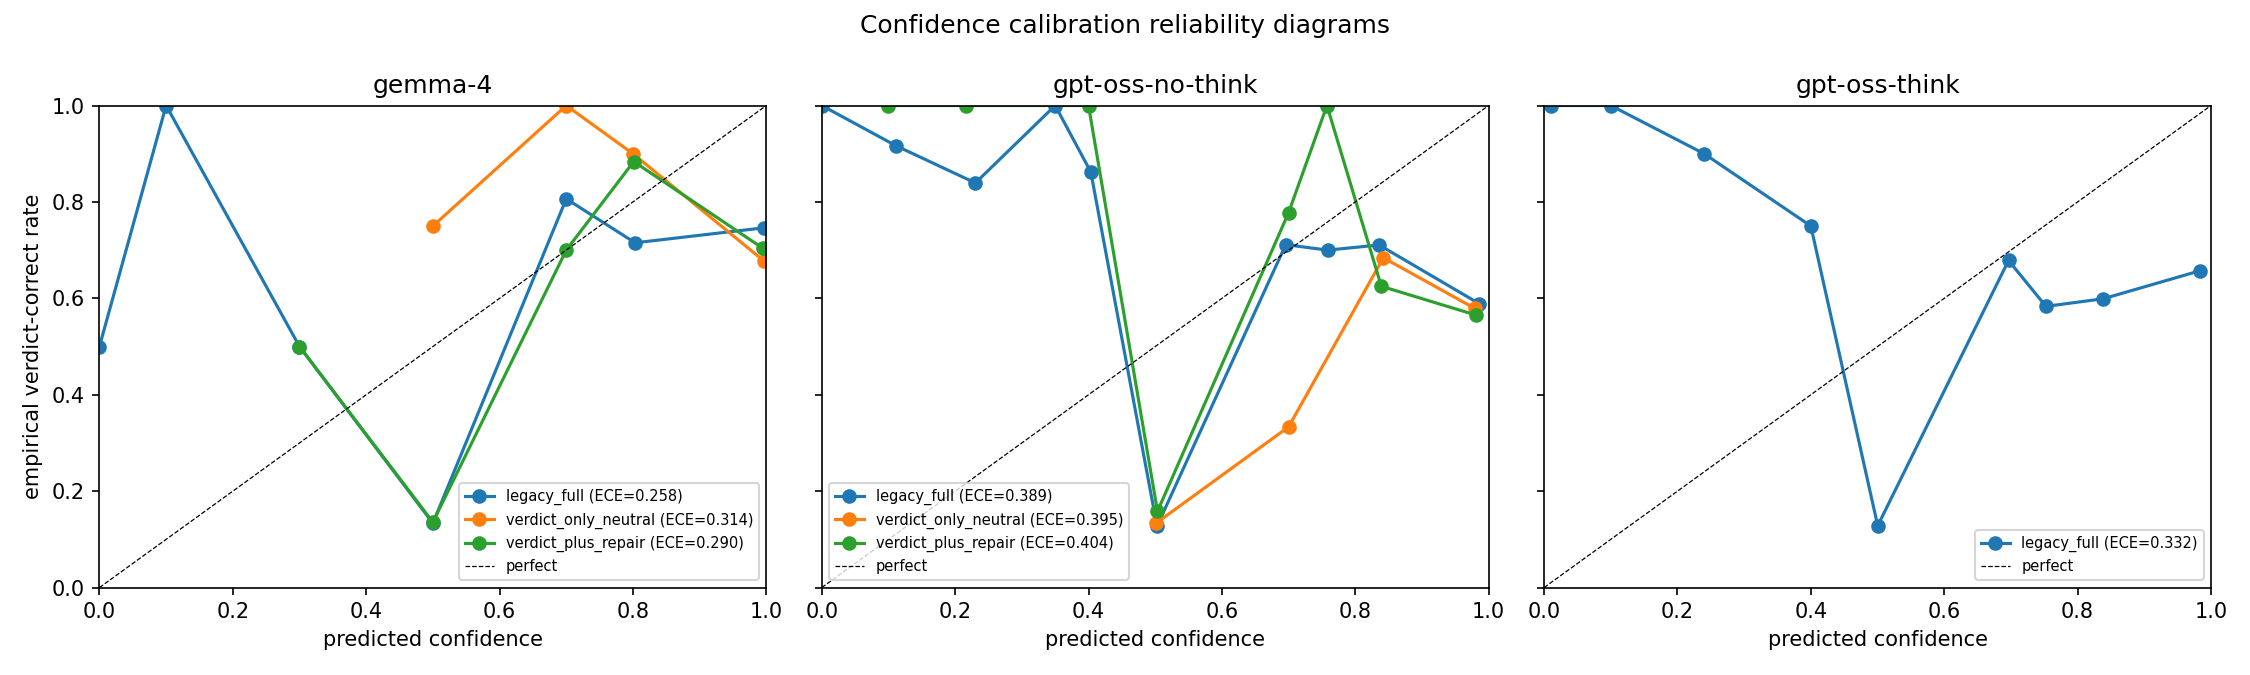
\includegraphics[width=\textwidth]{figures/fig8_reliability_diagram.png}
\caption{Reliability diagram for critic confidence. This diagnostic supports the interface-dependent calibration analysis in the main text rather than a standalone claim that LLM overconfidence is novel.}
\label{fig:appendix-calibration}
\end{figure*}

\end{document}
